\documentclass[a4paper, 8pt, twoside, openright]{book}
\usepackage[a4paper,top=4cm,bottom=2cm,left=2cm,right=2cm]{geometry}
\usepackage[english]{babel}
\usepackage[T1]{fontenc}
\usepackage[utf8]{inputenc}
\usepackage{fancyhdr}
\usepackage{float}
\usepackage{graphicx}
\usepackage{wrapfig}
\usepackage{siunitx} %per scrivere il simbolo °
\usepackage{verbatim} %per i commenti1
\usepackage{subfig}
\usepackage{amsmath}
\usepackage{algorithm}
\usepackage{algpseudocode}
\setcounter{secnumdepth}{3}
\setcounter{tocdepth}{6}
\usepackage{multirow}
\newcommand{\minitab}[2][l]{\begin{tabular}#1 #2\end{tabular}}
\usepackage{rotating}
\usepackage{xfrac}
\usepackage{cite}

\DeclareMathOperator*{\argmax}{arg\,max}
\DeclareMathOperator*{\argmin}{arg\,min}

%\usepackage{booktabs,array}
%\usepackage{tikz}

%\usepackage{tabularx}

%\usepackage{chngcntr}
%\counterwithin{table}{section}

%------------------------------ colors
\usepackage[usenames,dvipsnames,table]{xcolor} % use colors on table and more
\definecolor{333}{RGB}{51, 51, 51} % define custom color
\definecolor{background}{RGB}{248, 248, 255}
\definecolor{comment}{RGB}{17,167,5}
\definecolor{keyword}{RGB}{195,47,8}
\definecolor{string}{RGB}{142,195,0}
\definecolor{number}{RGB}{90,84,84}
\definecolor{identifier}{RGB}{0,90,201}

%------------------------------ source code
\usepackage{listings}

\lstset{
  basicstyle=\footnotesize\sffamily,
  commentstyle=\itshape\color{gray},
  captionpos=b,
  frame=shadowbox,
  language=HTML,
  rulesepcolor=\color{333},
  tabsize=2
}

\lstdefinestyle{code}{
  basicstyle=\footnotesize\sffamily,
  commentstyle=\color{comment},
}


%------------------------------ define Abstract environment, missing in the 'book' class
\newenvironment{abstract}{\cleardoublepage \null \vfill \begin{center}\bfseries\abstractname \end{center}}{\vfill\null}
\addto\captionsenglish{\renewcommand*\abstractname{Abstract}} % change Abstract title

%------------------------------ active url
\usepackage{url}
\renewcommand{\UrlFont}{\color{black}\small\ttfamily}
\usepackage{hyperref} % active ref
%------------------------------ macros
\newcommand{\sectionname}{Section} % define Section ref
\newcommand{\subsectionname}{Sub-section} % define Sub-section ref
\renewcommand*\arraystretch{1.4} % tables padding

%acronimi
\usepackage[printonlyused]{acronym}

\begin{document}
\frontmatter

\begin{titlepage} %------------------------------ TITLE PAGE
\begin{center}
\vbox to0pt{\vbox to\textheight{\vfill 
\includegraphics[width=11.5cm]{./Images/Background} \vfill}\vss}

\begin{center}
\begin{minipage}{.20\textwidth}
  
\includegraphics[height=2.5cm]{./Images/Icon4}
\end{minipage}\begin{minipage}{.45\textwidth}
  \begin{table}[H]
  \begin{tabular}{l}
  \scshape{\Large{\bfseries{Padua University}}} \\
  \hline \\
  \scshape{\Large{Engineering Course}} \\
  \end{tabular}
  \end{table}
\end{minipage}
\end{center}


\vspace{1cm}
\emph{\Large{Master~of~Computer~Engineering}} \\
\vspace{0.9cm}
\scshape{\Large{\bfseries{Computer Networks}}} \\
\vspace{0.2cm} \linespread{1} \scshape{\large{\bfseries{}}}
\end{center}

\vspace{12cm}
\begin{center}
Raffaele Di Nardo Di Maio
\end{center}

\vfill
\begin{center}
\hspace{-0.2cm}
\line(1, 0){360}\\
\textsc{Accademic Year 2019-2020}
\end{center}
\end{titlepage}


\cleardoublepage % make left page blank
\thispagestyle{empty} %------------------------------ DEDICA

\begin{comment}
\null
\vspace{2cm}
\begin{flushright}
//DEDICA
\end{flushright}
\vfill
\begin{quote}
  \textit{}
\end{quote}
\vfill
\null
\end{comment}

%\begin{abstract} %------------------------------ ABSTRACT
%\addcontentsline{toc}{chapter}{Abstract}
%\markboth{}{} % remove header
%\thispagestyle{empty}
%This is the abstract
%\end{abstract}

%\input{Chapters/Abstract.tex}
\begingroup %------------------------------ CONTENTS
  \makeatletter
  \let\ps@plain\ps@empty
  \makeatother
  \tableofcontents  
  \clearpage
\endgroup

\mainmatter

\chapter{OSI model}
The \textit{Open System Interconnection (OSI)} is the basic standardization of concepts related to networks (Figure \ref{OSI}). It was made by Internet \textit{Standard Organization (ISO)}. Each computer, connected as a node in the network, needs to have all OSI functionalities.
\begin{figure}[h]
\centering
\includegraphics[scale=0.4]{Images/OSI/OSI}\caption{\footnotesize{OSI model.}}\label{OSI}
\end{figure}

\section{Logical communication}
\begin{figure}[h]
\centering
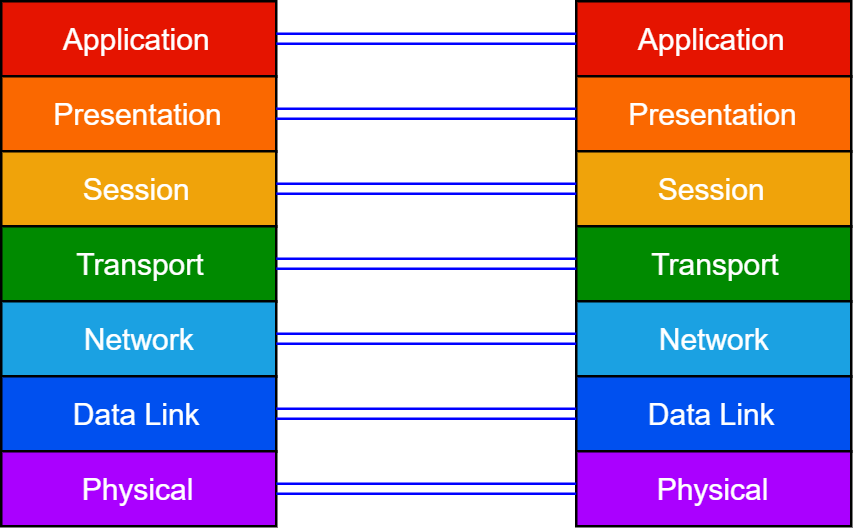
\includegraphics[scale=0.3]{Images/OSI/logic}
\end{figure}
Layer 1 is the only one in which the real connection is also the logic connection. Each layer is a module (black-box) that implements functionality (see Section \ref{onion_section}).

\section{Control plane}
\begin{figure}[h]
\centering
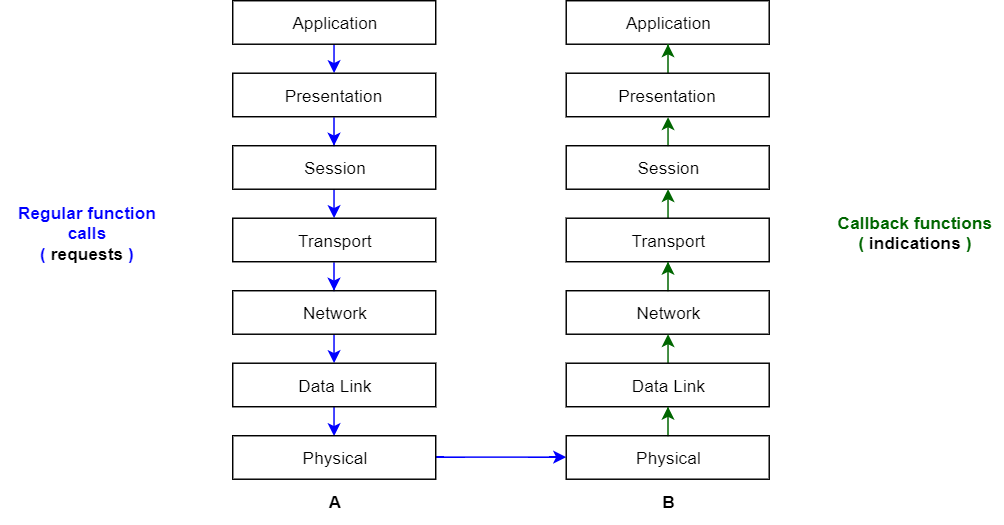
\includegraphics[scale=0.4]{Images/OSI/request_AB}
\caption{\footnotesize{Request from A to B.}}\label{requestAB}
\end{figure}
\begin{figure}[h]
\centering
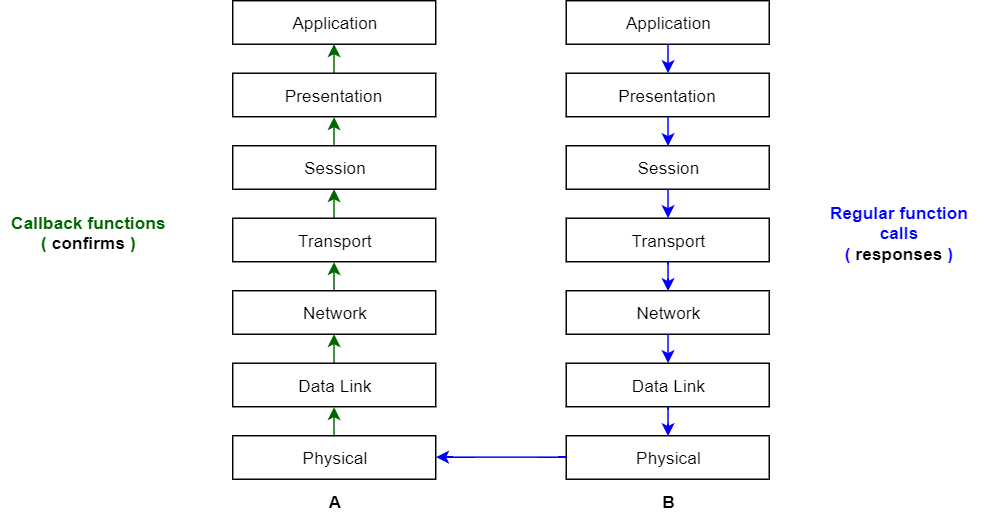
\includegraphics[scale=0.4]{Images/OSI/response_BA}
\caption{\footnotesize{Response from B to A.}}\label{responseBA}
\end{figure}
The control plane meaning comes from two words: "control" that is related to function activation and "plane", related to the geometry, because it's stacked in a sheet.\\
In OSI model, the \textit{direct connection} exists only between:
\begin{itemize}
\item{Upper and lower layers of the same device}
\item{Physical layers of different devices}
\end{itemize} 
From Figure \ref{requestAB} and Figure \ref{responseBA} we have seen two main types of function calls:
\begin{itemize}
\item{\textbf{Regular function calls}
\begin{itemize}
\item{library method invocations}
\item{system calls}
\item{HW enabled signals}
\end{itemize}
}
\item{\textbf{Callback functions}\\
the module of the upper layer is waken up by module of the lower layer.
\begin{itemize}
\item{OS signal handler\\
it asks library to call a function when something happens (EVENT-BASED PROGRAMMING)}
\item{Interrupt handlers}
\item{Blocking function calls\\
they start call but doesn't return if something doesn't happen}
\end{itemize}
}
\end{itemize}

\section{Data plane}
Data plane defines which data are shared among the network. Calling a function, we need to pass parameters to them (\textit{Data buffer}).\\
The PDU (Protocol Data Unit) of layer \textit{i+1} becomes the SDU (Service Data Unit), or payload, of lower Layer \textit{i}. Merging this payload, with the header of layer \textit{i}, we obtain the PDU of layer i (Figure \ref{pdu_sdu}). This procedure is called \textbf{encpsulation} (Figure \ref{encapsulation}).
\begin{figure}[h]
\centering
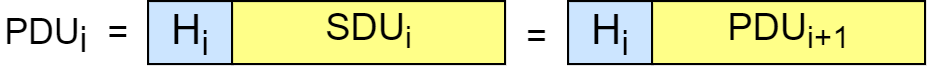
\includegraphics[scale=0.25]{Images/OSI/pdu_sdu}
\caption{PDU and SDU structure.}\label{pdu_sdu}
\end{figure}
\begin{figure}[h]
\centering
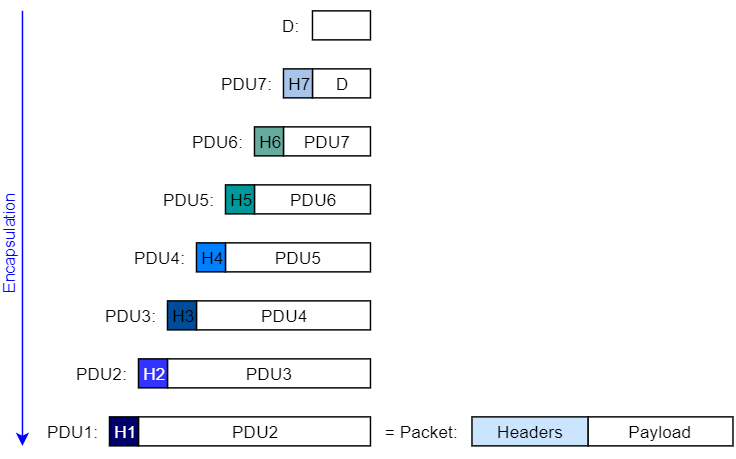
\includegraphics[scale=0.5]{Images/OSI/encapsulation}
\caption{\footnotesize{Encapsulation.}}\label{encapsulation}
\end{figure}
\vspace{3cm}
\section{Onion model}\label{onion_section}
The following image shows the layered structure of OS and computers and where OSI functionalities locations are highlighted. 
\begin{figure}[h]
\centering
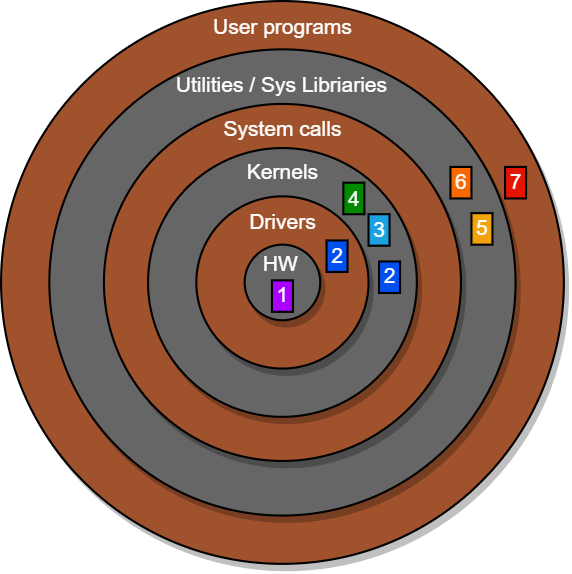
\includegraphics[scale=0.5]{Images/OSI/onion}
\caption{\footnotesize{Onion model.}}\label{onion}
\end{figure}

\section{TCP/IP Architecture}
The TCP/IP architecture is a reorganization of the previously mentioned OSI model (Figure \ref{OSI}) and it composes the main structure of the Internet Protocol. 
\begin{figure}[h]
\centering
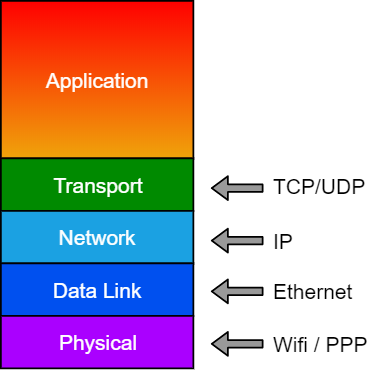
\includegraphics[scale=0.5]{Images/OSI/tcp_ip}
\end{figure}

\section{Application paradigms}
\subsection{Client-Server}
It's based on the presence of two main entities:
\begin{itemize}
\item{\textbf{Client =} active entity\\
it generates the request
}
\item{\textbf{Server =} passive entity\\
it's waiting for client requests and when it receives it, it only replies to it.
}
\end{itemize}
The main characteristic of this paradigm is the \textbf{"immediate" response time}, that is the time between the arrival of the request by the client and the reply with the generate response.\\
To send the request, the client needs to know:
\begin{itemize}
\item{server name}
\item{how to reach it}
\item{what data is required on server (trackable)}
\end{itemize}
\begin{figure}[h]
\centering
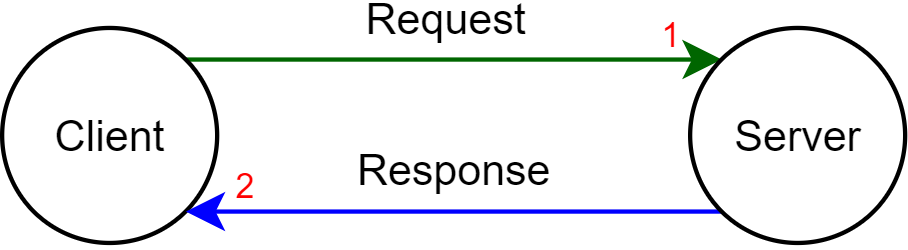
\includegraphics[scale=0.25]{Images/OSI/client_server}
\caption{\footnotesize{Client-Server architecture.}}\label{cs}
\end{figure}

\subsection{Peer-to-Peer (P2P)}
Its diffusion started at first years of XXI century. It's used to share media. Each node in the network can be client (making requests) or server (replying to requests).\\
In Figure \ref{p2p}, $USER_1$ doesn't know which is the user in the network that shared the content. Hence, he sends the request for the content to a node in the network and this one can reply with two possible responses:
\begin{itemize}
\item{\textbf{C=} content (media)}
\item{\textbf{R=} reference to another node (that has the required content or knows which node has the content)}
\end{itemize}
Each node can also forward the request to some other node and so it becomes the intermediary of the communication.
\begin{figure}[h]
\centering
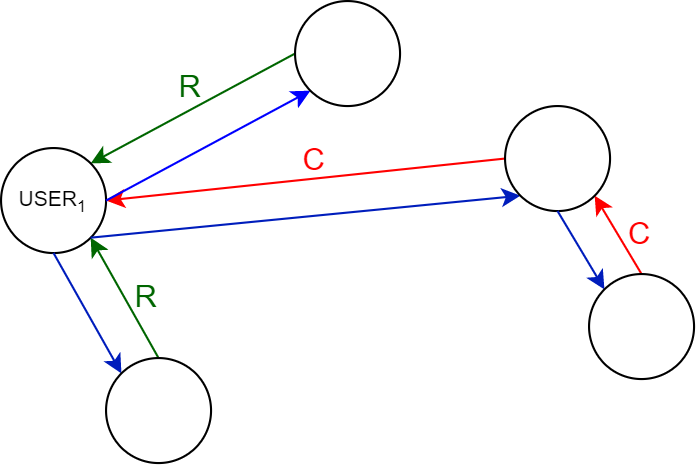
\includegraphics[scale=0.35]{Images/OSI/p2p}
\caption{\footnotesize{P2P architecture.\\}}\label{p2p}
\end{figure}

\subsection{Publish/Subscribe/Notify}
The subscriber subscribes to the dispatcher (notifier) a set of messages that wants to be notified. The notifier usually filters the messages that it receives and, when there are new messages that respect the subscription of the user, notify them to the user.\\ The messages comes \textit{asynchronously} to the dispatcher. There is no \textit{Polling} made periodically by the user (there isn't Busy Waiting). There are some applications, like Whatsapp, that work in this way but in the past, this app made by Facebook doesn't really work asynchronously. In fact there was a polling policy.
\begin{figure}[H]
\centering
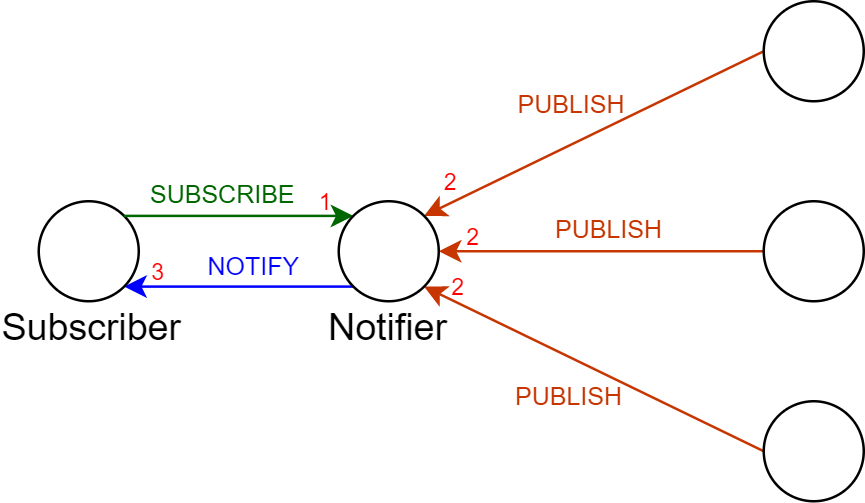
\includegraphics[scale=0.35]{Images/OSI/publish_subscribe}
\caption{\footnotesize{Publish/Subscribe/Notify architecture.}}\label{publish_subscribe}
\end{figure}

\section{Types of packets}
\begin{figure}[H]
\centering
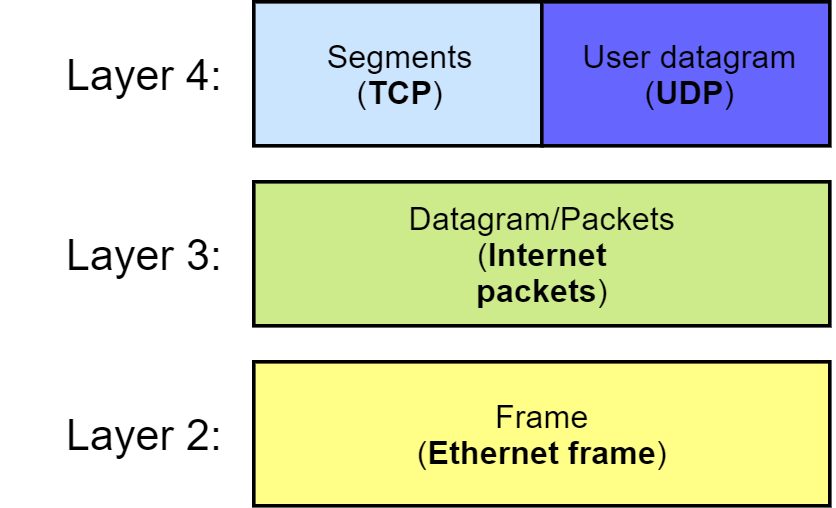
\includegraphics[scale=0.28]{Images/OSI/packets}
\caption{\footnotesize{Standard names of packets.}}\label{packets}
\end{figure}
TCP connection works at Layer 4 but at upper layers, it seems to work as a stream. In TCP connection, it is usually specified the port number, that is the upper layer protocol specification (Layer 5).

\chapter{Application Layer}
\chapter{C programming}
The C is the most powerful language and also can be considered as the language nearest to Assembly language. Its power is the speed of execution and the easy interpretation of the memory.\\
C can be considered very important in Computer Networks because it doesn't hide the use of system calls. Other languages made the same thing, but hiding all the needs and evolution of Computer Network systems.

\section{Organization of data}\label{littleBig}
Data are stored in the memory in two possible ways, related to the order of bytes that compose it. There are two main ways, called Big Endian and Little Endian.
\begin{center}
\begin{tabular}{c}
\begin{lstlisting}[linewidth=30pt, basicstyle=\footnotesize\sffamily,]
int i;
\end{lstlisting}
\end{tabular}
\end{center}

\begin{figure}[h]
\centering
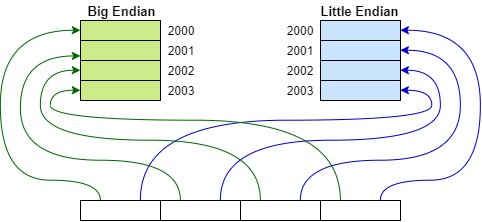
\includegraphics[scale=0.68]{Images/Programming/endians}
\caption{\footnotesize{Little Endian and Big Endian.}}
\end{figure}

The order of bytes in packets, sent through the network, is Big Endian.\\
The size of \textbf{int, float, char, ...} types
depends on the architecture used. The max size of possible types depends on the architecture (E.g. in 64bits architecture, in one istruction, 8 bytes can be written and read in parallel).

\begin{table}[h]
\centering
\begin{tabular}{|c|c|}
\hline
\textbf{signed}&{unsigned}\\
\hline
{int8\_t}&{uint8\_t}\\
{int16\_t}&{uint16\_t}\\
{int32\_t}&{uint32\_t}\\
{int64\_t}&{uint64\_t}\\
\hline
\end{tabular}\caption{<stdint.h>}
\end{table}
\vspace{4cm}
\section{Struct organization of memory}
The size of a structure depends on the order of fields and the architecture. This is caused by alignment that depends on the number of memory banks, number of bytes read in parallel. For example the size is 4 bytes for 32 bits architecture, composed by 4 banks (Figure \ref{parallel}). The Network Packet Representation is made by a stream of 4 Bytes packets as we're using 32 bits architecture. 
\begin{center}
\begin{tabular}{c}
\begin{lstlisting}[linewidth=200pt, basicstyle=\footnotesize\sffamily,]
struct example1        struct example2
{                      {
	char c;	               int x;
	int x;	               char c;
}                      }
\end{lstlisting}
\end{tabular}
\end{center}

\begin{figure}[h]
\centering
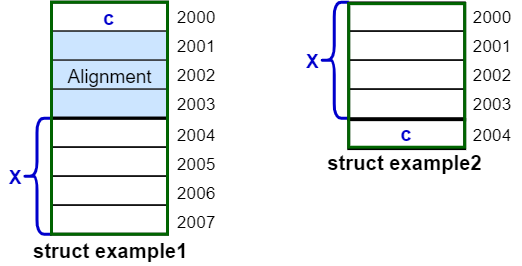
\includegraphics[scale=0.5]{Images/Programming/struct}
\end{figure}

\begin{figure}[h]
\centering
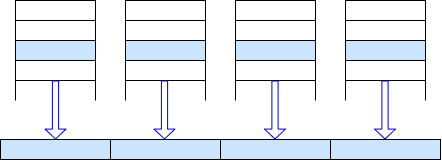
\includegraphics[scale=0.68]{Images/Programming/parallel_reading}
\caption{\footnotesize{Parallel reading in one istruction in 32 bits architecture.}}\label{parallel}
\end{figure}

\vspace{3cm}
\section{Structure of C program}
The program stores the variable in different section (Figure \ref{program}):
\begin{itemize}
\item{\textbf{Static area}\\
where global variables and static library are stored, it's initialized immediately at the creation of the program. Inside this area, a variable doesn't need to be initialized by the programmer because it's done automatically at the creation of the program with all zeroes.}
\item{\textbf{Stack}\\
allocation of variables, return and parameters of functions}
\item{\textbf{Heap}\\
dinamic allocation }
\end{itemize}

\begin{figure}[h]
\centering
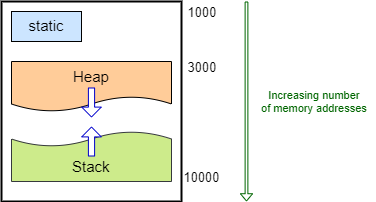
\includegraphics[scale=0.68]{Images/Programming/program}
\caption{\footnotesize{Structure of the program.}}\label{program}
\end{figure}
\chapter{Network services in C}
\section{Application layer}
We need IP protocol to use Internet. In this protocol, level 5 and 6 are hidden in Application Layer.\\
In this case, Application Layer needs to interact with Transport Layer, that is implemented in OS Kernel (Figure \ref{app_kernel}). Hence Application and Transport can talk each other with System Calls.
\begin{figure}[h]
\centering
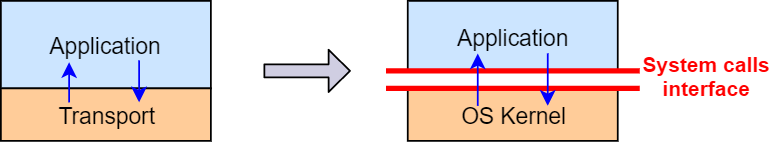
\includegraphics[scale=0.6]{Images/NetworkC/application}\caption{\footnotesize{System calls interface.}}\label{app_kernel}
\end{figure}

\section{socket}\label{socket}
Entry-point (system call) that allow us to use the network services. It also allows application layer to access to level 4 of IP protocol. 
\begin{center}
\begin{tabular}{c}
\begin{lstlisting}[linewidth=270pt, basicstyle=\footnotesize\sffamily,]
#include <sys/types.h>
#include <sys/socket.h>

int socket(int domain, int type, int protocol);\\
\end{lstlisting}
\end{tabular}
\end{center}

\begin{table}[h]
\centering
\begin{tabular}{rcl}
\textbf{RETURN VALUE} & \multicolumn{2}{l}{\textit{File Descriptor (FD) of the socket} }\\
{} & \multicolumn{2}{l}{\textit{-1} if some error occurs and errno is set appropriately}\\
{} & \multicolumn{2}{l}{(You can check value of errno including <errno.h>).}\\
\end{tabular}
\end{table}

\begin{table}[h]
\centering
\begin{tabular}{rcl}
\textbf{domain =} & \multicolumn{2}{l}{\textit{Communication domain}}\\
{} & \multicolumn{2}{l}{protocol family which will be used for communication.}\\
{} & \textbf{AF\_INET:} & {IPv4 Internet Protocol}\\
{} & \textbf{AF\_INET6:} & {IPv6 Internet Protocol}\\
{} & \textbf{AF\_PACKET:} & {Low level packet interface}\\
& &\\
\textbf{type =} & \multicolumn{2}{l}{\textit{Communication semantics}}\\
{} & \textbf{SOCK\_STREAM:} & {Provides sequenced, reliable, two-way, connection-based}\\
{} & {} & {bytes stream. An OUT-OF-BAND data mechanism may}\\
{} & {} & {be supported.}\\
{} & \textbf{SOCK\_DGRAM} & {Supports datagrams (connectionless, unreliable messages} \\
& & {of a fixed maximum length).}\\
& & \\
\textbf{protocol =} & \multicolumn{2}{l}{\textit{Particular protocol to be used within the socket}}\\
{} & \multicolumn{2}{l}{Normally there is only a protocol for each socket type and protocol}\\
{} & \multicolumn{2}{l}{family (protocol=0), otherwise ID of the protocol you want to use}\\
\end{tabular}
\end{table}

\vspace{10cm}
\section{TCP connection}
In TCP connection, defined by type \textbf{SOCK\_STREAM} as written in the Section \ref{socket}, there is a client that connects to a server. It uses three primitives (related to File System primitives for management of files on disk) that do these logic actions:
\begin{enumerate}
\item{start (open bytes stream)}
\item{add/remove bytes from stream}
\item{finish (clos bytes stream)}
\end{enumerate}
TCP is used transfering big files on the network and for example with HTTP, that supports parallel download and upload (FULL-DUPLEX). The length of the stream is defined only at closure of the stream.
 
\subsection{Client}
\subsubsection{connect}
The client calls \textbf{connect()} function, after \textbf{socket()} function of Section \ref{socket}. This function is a system call that client can use to define what is the remote terminal to which he wants to connect.

\begin{center}
\begin{tabular}{c}
\begin{lstlisting}[linewidth=370pt, basicstyle=\footnotesize\sffamily,]
#include <sys/types.h>
#include <sys/socket.h>

int connect(int sockfd, const struct sockaddr *addr,socklen_t addrlen);
\end{lstlisting}
\end{tabular}
\end{center}

\begin{table}[h]
\centering
\begin{tabular}{rcl}
\textbf{RETURN VALUE} & \multicolumn{2}{l}{\textit{0} if connection succeds}\\
{} & \multicolumn{2}{l}{\textit{-1} if some error occurs and errno is set appropriately}\\
& & \\
\textbf{sockfd =} & \multicolumn{2}{l}{\textit{Socket File Descriptor} returned by socket().}\\
& &\\
\textbf{addr =} & \multicolumn{2}{l}{\textit{Reference to struct sockaddr}}\\
{} & \multicolumn{2}{l}{sockaddr is a general structure that defines the concept of address.}\\
{} & \multicolumn{2}{l}{In practice it's a union of all the possible specific structures of each protocol.}\\
{} & \multicolumn{2}{l}{This approach is used to leave the function written in a generic way.}\\
& & \\
\textbf{addr =} & \multicolumn{2}{l}{\textit{Length of specific data structure used.}}\\
\end{tabular}
\end{table}
\vspace{8cm}
In the following there is the description of struct \textbf{sockaddr\_in}, that is the specific sockaddr structure implemented for family of protocls \textbf{AF\_INET}:

\begin{center}
\begin{tabular}{c}
\begin{lstlisting}[linewidth=350pt, basicstyle=\footnotesize\sffamily,]
#include <netinet/in.h>

struct sockaddr_in {
    sa_family_t    sin_family; /* address family: AF_INET */
    in_port_t      sin_port;   /* port in network byte order */
    struct in_addr sin_addr;   /* internet address */
};

/* Internet address. */
struct in_addr {
    uint32_t       s_addr;     /* address in network byte order */
};\\
\end{lstlisting}
\end{tabular}
\end{center}
As mentioned in Section \ref{littleBig}, network data are organized as Big Endian, so in this case we need to insert the IP address according to this protocol. It can be done as in previous example or with the follow function:
\begin{center}
\begin{tabular}{c}
\begin{lstlisting}[linewidth=280pt, basicstyle=\footnotesize\sffamily,]
#include <sys/socket.h>
#include <netinet/in.h>
#include <arpa/inet.h>

int inet_aton(const char *cp, struct in_addr *inp);
\end{lstlisting}
\end{tabular}
\end{center}
The port number is written according to Big Endian architecture, through the next function:
\begin{center}
\begin{tabular}{c}
\begin{lstlisting}[linewidth=200pt, basicstyle=\footnotesize\sffamily,]
#include <arpa/inet.h>

uint16_t htons(uint16_t hostshort);
\end{lstlisting}
\end{tabular}
\end{center}

\subsubsection{write()}
Application protocol uses a readable string, to excange readable information (as in HTTP). This tecnique is called simple protocol and commands, sent by the protocol, are standardized and readable strings.  

\begin{center}
\begin{tabular}{c}
\begin{lstlisting}[linewidth=280pt, basicstyle=\footnotesize\sffamily,]
#include <unistd.h>

ssize_t write(int fd, const void *buf, size_t count);
\end{lstlisting}
\end{tabular}
\end{center}

\begin{table}[h]
\centering
\begin{tabular}{rcl}
\textbf{RETURN VALUE} & \multicolumn{2}{l}{\textit{Number of bytes written} on success}\\
{} & \multicolumn{2}{l}{\textit{-1} if some error occurs and errno is set appropriately}\\
& & \\
\textbf{fd =} & \multicolumn{2}{l}{\textit{Socket File Descriptor} returned by socket().}\\
& &\\
\textbf{buf =} & \multicolumn{2}{l}{\textit{Buffer of characters to write}}\\
& & \\
\textbf{count =} & \multicolumn{2}{l}{\textit{Max number of bytes to write} in the file (stream).}\\
\end{tabular}
\end{table}
\vspace{4cm}
The write buffer is usually a string but we don't consider the null value (\textbf{$\backslash 0$} character), that determine the end of the string, in the evaluation of count (\textbf{strlen(buf)-1}). This convention is used because \textbf{$\backslash 0$} can be part of characters stream.\\

\subsubsection{read()}
The client uses this blocking function to wait and obtain response from the remote server. Not all the request are completed immediat from the server, for the meaning of stream type of protocol. Infact in this protocol, there is a flow for which the complete sequence is defined only at the closure of it\ref{socket}.\\
\textbf{read()} is consuming bytes fom the stream asking to level 4 a portion of them, because it cannot access directly to bytes in Kernel buffer. Lower layer controls the stream of information that comes from the same layer of remove system.\\

\begin{center}
\begin{tabular}{c}
\begin{lstlisting}[linewidth=280pt, basicstyle=\footnotesize\sffamily,]
#include <unistd.h>

       ssize_t read(int fd, void *buf, size_t count);
\end{lstlisting}
\end{tabular}
\end{center}

\begin{table}[h]
\centering
\begin{tabular}{rcl}
\textbf{RETURN VALUE} & \multicolumn{2}{l}{\textit{Number of bytes read} on success}\\
{} & \multicolumn{2}{l}{\textit{0} if EOF is reached (end of the stream)}\\
{} & \multicolumn{2}{l}{\textit{-1} if some error occurs and errno is set appropriately}\\
& & \\
\textbf{fd =} & \multicolumn{2}{l}{\textit{Socket File Descriptor} returned by socket().}\\
& &\\
\textbf{buf =} & \multicolumn{2}{l}{\textit{Buffer of characters in which it reads and stores info}}\\
& & \\
\textbf{count =} & \multicolumn{2}{l}{\textit{Max number of bytes to read} from the file (stream).}
\end{tabular}
\end{table}
So if \textbf{read()} doesn't return, this means that the stream isn't ended but the system buffer is empty.\\
If \textbf{read=0}, the function met EOF and the local system buffer is now empty. This helps client to understand that server ended before the connection.

\begin{figure}[h]
\centering
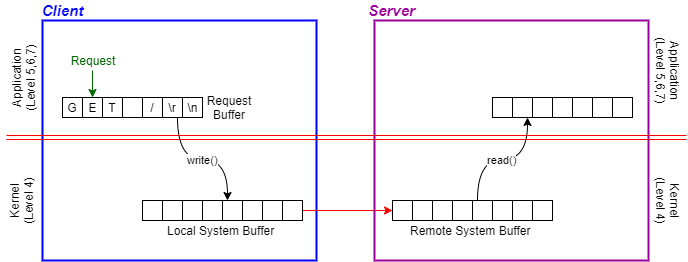
\includegraphics[scale=0.6]{Images/NetworkC/read_write1}\caption{\footnotesize{Request by the client.}}\label{rw1}
\end{figure}

\begin{figure}[h]
\centering
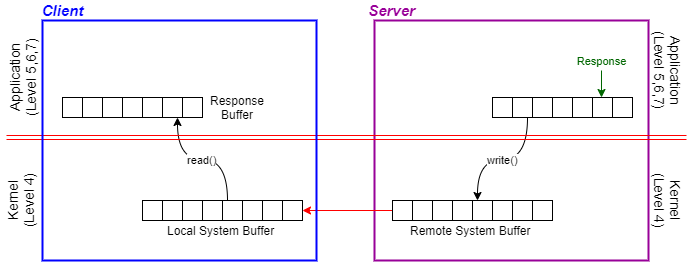
\includegraphics[scale=0.6]{Images/NetworkC/read_write2}\caption{\footnotesize{Response from the server.}}\label{rw2}
\end{figure}

\clearpage
\subsubsection{Client connection to google}
The following piece of code define a structure, used to connect to Google server. 
\lstinputlisting[caption={\footnotesize{web\_client.c}}, style=code, firstnumber=1, firstline=1, lastline=73, label=web_client, language=c]{../src/2_tcp/web_client.c}

The most important thing is that \textbf{socket()} is entry-point for level 4, but also \textbf{connect()} is the request to Kernel to extablish the connection.\\ \textbf{read()} and \textbf{write()} are system calls used respectively to obtain result(response) of a request and to generate request.\\ These function permit us to ask to lower level to do this things, without knowing content of system buffers (stream).

\section{UDP connection}
UDP connection is defined by type \textbf{SOCK\_DGRAM} as specified in Section \ref{socket}. It's used for application in which we use small packets and we want immediate feedback directly from application. It isn't reliable because it doesn't need confirmation in transport layer. It's used in Twitter application and in video streaming.  
\chapter{Gateway}
A gateway is a device that forwards messages from another device, the client, to a second device, the server or another gateway.
In the following figures, there are two examples of gateways: Layer-3 gateways (routers in Section \ref{router_section}) and Layer-7 gateways (proxy).
\begin{figure}[h]
\centering
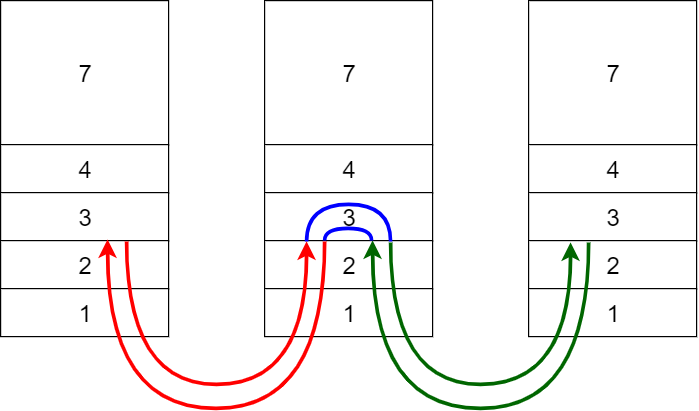
\includegraphics[scale=0.4]{Images/Gateway/gateway_3}
\caption{\footnotesize{Router (Layer-3 gateway).}}\label{gateway_3}
\end{figure}
\begin{figure}[h]
\centering
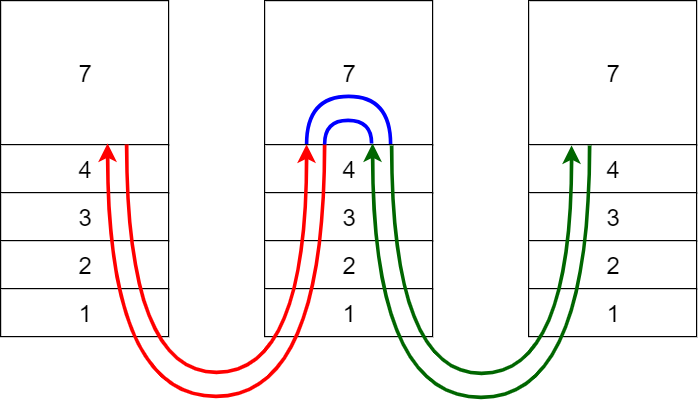
\includegraphics[scale=0.4]{Images/Gateway/gateway_7}
\caption{\footnotesize{Proxy (Layer-7 gateway).}}\label{gateway_7}
\end{figure}

\section{Proxy}
A Layer-7 gateway is also called proxy. It works as an intermediary between two identical protocols (Figure \ref{proxy}). Instead of Layer-3 gateways, proxy can also see the full stream of data, analyze HTTP headers and implement new functions. 
\begin{figure}[h]
\centering
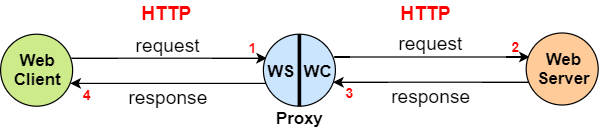
\includegraphics[scale=0.42]{Images/Gateway/proxy}
\caption{\footnotesize{Example of proxy use.}}\label{proxy}
\end{figure}
The main possible functions are:
\begin{itemize}
\item{\textbf{Caching}\\
It's used to reduce traffic directed to the server. The proxy does the most expensive job, managing all the requests of the same page of the server. \\
After the request of the page for the first time, the proxy asks the page to the server and then stores in its system, before replying. Hence the next clients requests of the same page will be manage only by proxy because the page was already stored in its system.\\
In this case the server needs to manage only a request by proxy and provide a response to proxy.
\begin{figure}[h]
\centering
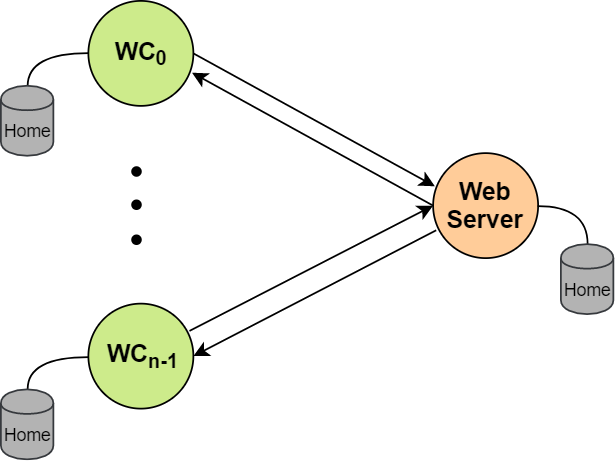
\includegraphics[scale=0.38]{Images/Gateway/proxy_cache_no}
\caption{\footnotesize{Example of caching without proxy.}}\label{proxy_cache_no}
\end{figure}
\begin{figure}[h]
\centering
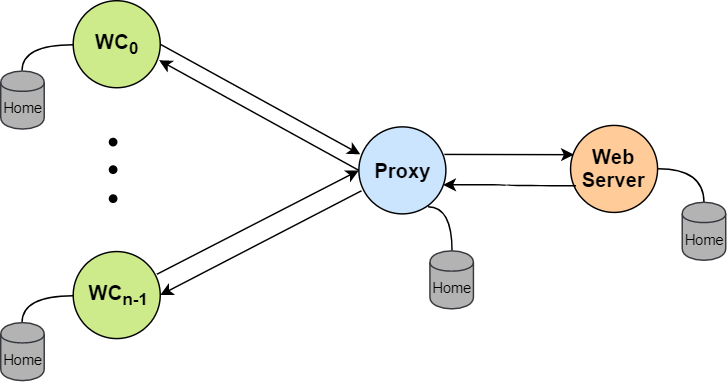
\includegraphics[scale=0.4]{Images/Gateway/proxy_cache}
\caption{\footnotesize{Example of caching using proxy.}}\label{proxy_cache}
\end{figure}
}
\item{\textbf{Filtering}\\
The proxy can do two actions:
\begin{itemize}
\item{\textbf{Filtering the requested resource by the client}\\
there are many companies that doesn't give access to some services (E.g. no access to Facebook, Youtube, ...).\\
We cannot use a filtering approach at lower levels because in some cases clients can access to services through intermediate addresses, different from the one we want to reach. Hence we need to analyze the HTTP request at upper layer.}
\item{\textbf{Filtering the content of the response}\\
for parent control approach.}
\end{itemize}
\begin{figure}[h]
\centering
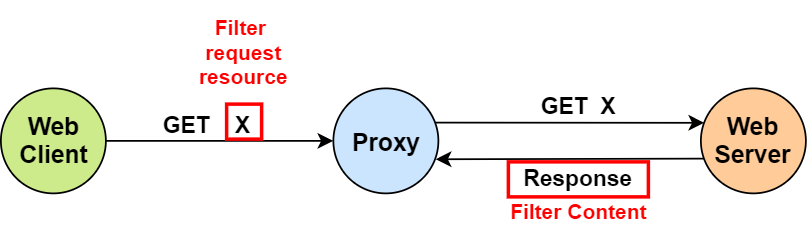
\includegraphics[scale=0.4]{Images/Gateway/proxy_filter}
\caption{\footnotesize{Example of proxy filtering.}}\label{proxy_filter}
\end{figure}
}
\item{\textbf{Web Application Firewall (WAF)}\\
The proxy is specialized and used to block suspicious requests. This is done by analyzing request content, looking for not secure pattern.\\
A possible pattern can be \textit{".."} in the path of the resource, that could give access to not accessible part of the File System (injection). Another possible pattern could be a suspicious parameter for a web application to manage SQL database (SQL injection).
\begin{figure}[h]
\centering
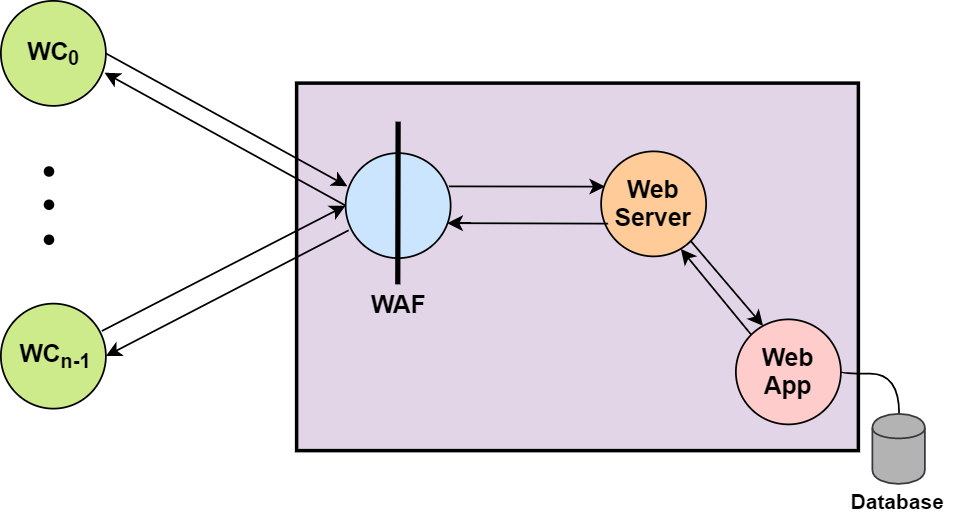
\includegraphics[scale=0.4]{Images/Gateway/proxy_waf}
\caption{\footnotesize{Example of WAF use.}}\label{proxy_waf}
\end{figure}
}
\item{\textbf{Load Balancing}\\
The proxy is a load balancer for the clients requests to the server.\\
There are many servers to manage requests by client. The client makes the request of the web page but in the reality it's talking with the proxy, that manage the request by sending it to a particular server.\\
This action is repeated for each client's request. Hence the client thinks that is talking to one server but in reality, the proxy distribute the requests among several servers. 
\begin{figure}[h]
\centering
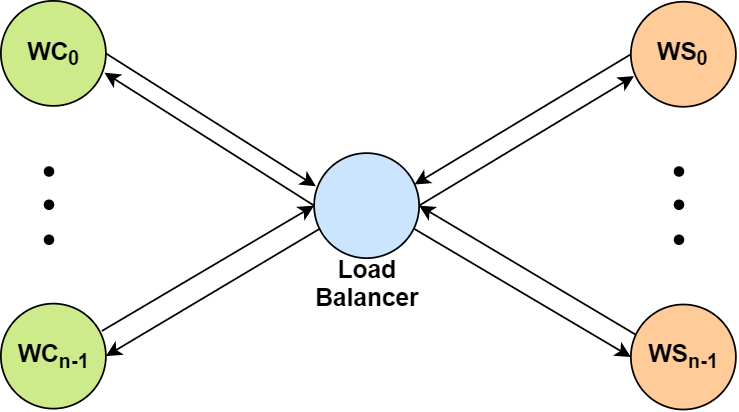
\includegraphics[scale=0.4]{Images/Gateway/proxy_load}
\caption{\footnotesize{Example of load balancing through proxy.}}\label{proxy_load}
\end{figure}
}
\end{itemize}

\section{Router} \label{router_section}
A router is a device that does two main functions:
\begin{enumerate}
\item{\textbf{Routing}\\
it decides on which outbound link send the packet. This decision is based on destination address and its router table (Table \ref{routing_table}). In each routing table, a network address is associated to an outbound interface, where the packet will be forwarded.\\
Each network address is followed by a \textbf{"/"} and a number that defines how many most significant bits of \textbf{net mask} are set to 1. The default adddress, that is always in each routing table, is \textbf{0.0.0.0}. This one is associated to the interface on which the packet will be sent if no one of the previous messages matches with the one of the destination.\\
For each entry of the routing table, the network address is ANDed with its net mask and the IP address, we are looking for, ANDed with that net mask gives us the same result of the first one, the packet is sent to the corresponding interface.\\
The default address \textbf{0.0.0.0} is associated with a net mask, composed by all 0's. Hence every address, ANDed with this net mask, matches with default address \textbf{0.0.0.0}.
\begin{table}[h]
\centering \footnotesize
\begin{tabular}{|c|c|}
\hline
\textbf{Address prefix} & \textbf{Outbound interface}\\
\hline
{147.162.0.0\textit{/16}} & {2}\\
{88.80.187.0\textit{/24}} & {4}\\
{...} & {...}\\
{0.0.0.0} & {1}\\
\hline
\end{tabular}
\caption{Example of a routing table.}\label{routing_table}
\end{table}
}
\item{\textbf{Switching}\\
it sends the packet to the link previously selected.}
\end{enumerate}
Each router manages all the incoming packets, storing them in a input \textbf{FIFO buffer} (\textit{Standard Service Local}).By default, if packets arrive too fast to in the buffer, w.r.t. velocity of incoming data processing, new packets are dropped if buffer is already full according to some policy (Figure \ref{}).\\
Hence routers has not responsability if some packets are dropped because of it declares it in advance and its goal is to give user the best effort. The behaviour of the router management of the input buffer is based on different policy, according to a goal:\\
\begin{itemize}
\item{\textit{To reduce} \textbf{latency}\\
the packets are sorted by precedence index
}
\item{\textit{To reduce} \textbf{loss rate}\\
dropped packets are the last enetered without \textit{R} bit set
}
\item{\textit{To reduce} \textbf{throughput}\\
the packets are stored by index, calculated by the router, based on the amount of data transfered from each source/destination in a time unit (e.g. RSUP, virtual clock, MPLS, Stop \& GO criteria)
}
\end{itemize}
The user cannot set all the possible criteria, because these depend from agreement developed with Service Provider. Hence the Internet Service Provider, if all criteria are set, reset them all before sending packets to Internet.
\chapter{Internet Protocol}\label{layer3}
The Internet protocol was the result of research job made by american Department of Defence (DoD). \textit{Internet} means Inter-networks communication and was designed for use of interconnected systems of packet-switched computer communication networks. The only things in common between the networks is the packet architecture.\\
Today the Internet Protocol is the only one yet used in Layer 3. The Internet Protocol provides transmission of blocks of data called datagrams, from sources to destinations, where sources and destinations are hosts identified by fixed length addresses \cite{RFC791}.\\
The two main functions, that Internet Protocol needs to provide, are:
\begin{enumerate}
\item{\textbf{Definition of unified addresses (Section \ref{ip_section})}}
\item{\textbf{Fragmentation (Section \ref{fragment_section})}}
\end{enumerate}
The creation of Internet Protocol comes from the needs of interconnection between networks (Figure \ref{net_structure}). Each network has its own protocol and it's composed by serveral devices, connected each other. The terminal devices of a network are the hosts and they can talk to others in the net through routers.\\
The new devices added with the invention of Internet Protocol were the Gateways, devices similar to routers that also translate protocols of different networks. The links inside the network (that connects routers and hosts) work on Layer 3 and the links between gateways work as Layer 2 networks, that doesn't required routing function.\\
Nowadays, networks are almost local so the gateways work mostly as routers. In fact, the routers don't exist as their definition tells (Figure \ref{lan}). The routing mechanism is no more done at Layer-3 but at Layer-2.\\
Ping is the most known service of Internet Protocol.
\begin{figure}[h]
\centering
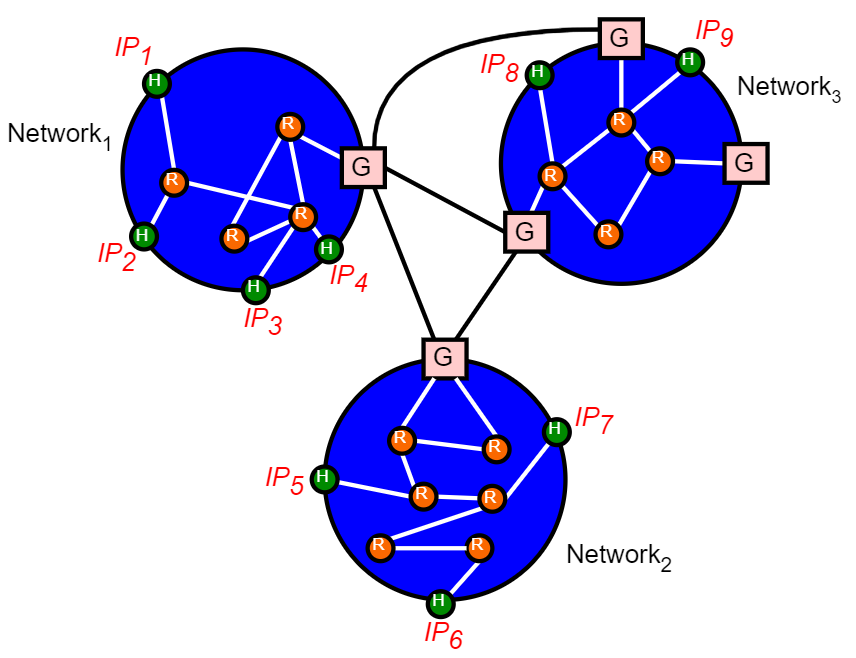
\includegraphics[scale=0.4]{Images/IP/net_structure}
\caption{\footnotesize{Internet structure.}}\label{net_structure}
\end{figure}
\begin{figure}[h]
\centering
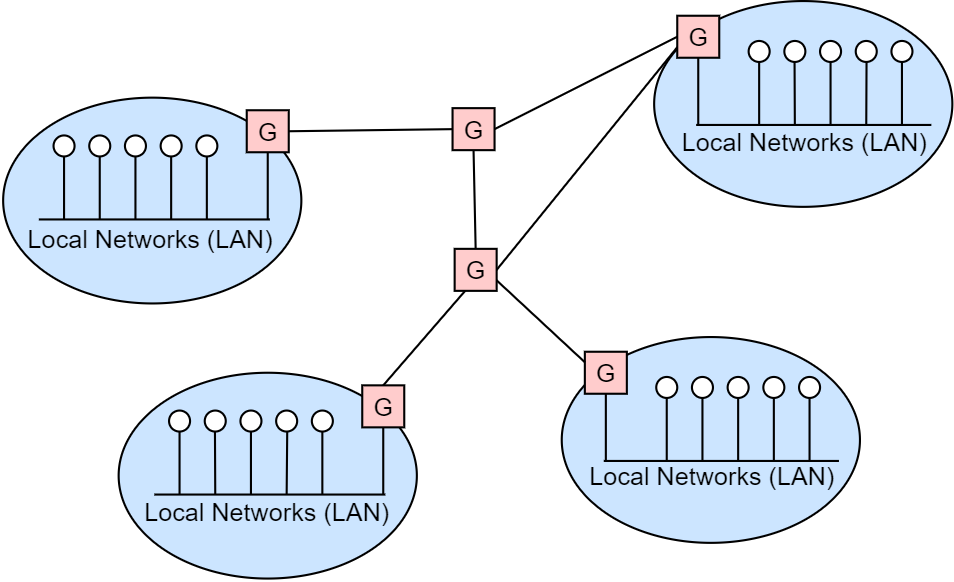
\includegraphics[scale=0.4]{Images/IP/lan}
\caption{\footnotesize{LAN structure.}}\label{lan}
\end{figure}
\clearpage
\section{Terminology}
\begin{itemize}
\item{\textbf{Round Trip Time (RTT)}\\
time needed from network to send the packet and receive the response packet
}
\item{\textbf{Delay}\\
passed time before the true service
}
\item{\textbf{Bit rate (Bandwidth)}\\
amount of Bit/s or Bytes/s of the network
}
\item{\textbf{Throughput}\\
amount of data/s that I can really transmit
}
\item{\textbf{Relaibility}\\
capacity of being reliable and losing few packets. It's related to inverse of:
$$loss\;\;rate = \frac{\#\;lost\;packets}{\#\;sent\;packets}$$
}
\end{itemize}

\section{IP address}\label{ip_section}
To send packets among different networks, we need to identify gloabally the destination host and IP address was designed to solve this problem. The IP addresses are 32 bits numbers. They are commonly represented as a set of 4 numbers separated by a point and each of them is the decimal representation of the corresponding byte in the IP address.\\
An IP address can be divided into two parts: Network part and Host part. In the past, the IP addresses were classified by three main classes, based on the size of their Network part: \textit{Class A, Class B, Class C} (Figure \ref{classes_ip}).\\
This classification of addresses in this way isn't very efficient because this cannot manage well addressing of large number of small networks or small number of large networks.\\
To do it it was introduced the Net Mask, a bit mask composed by a sequence of 1's followed by 0's, that permits us to define the parts of an address of whatever dimension we want (Figure \ref{netmask}). This is useful also to create subnetworks of a given set of hosts (Figure \ref{dei_ip}).\\
There are also two special addresses:
\begin{itemize}
\item{\textbf{Network address (no hosts)}\\
Host part = \textit{0...0000}
}
\item{\textbf{Broadcast address (all hosts in the network)}\\
Host part = \textit{1...1111}
}
\end{itemize}
Hence to give an address to each endpoint of a \textbf{Point To Point} link, we need to use at least an Host part of 2 bits (Figure \ref{point2point}).  
\begin{figure}[h]
\centering
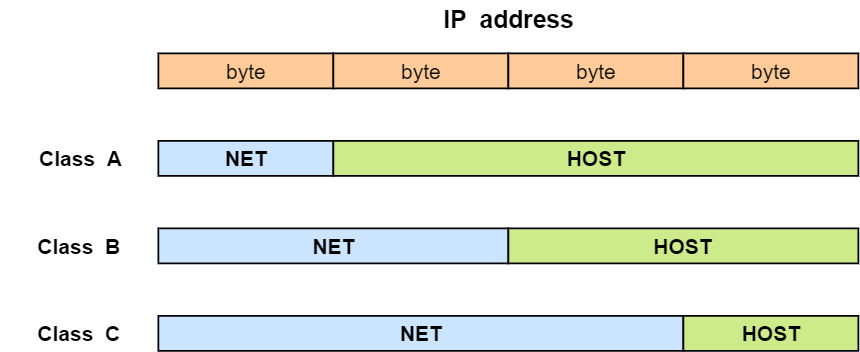
\includegraphics[scale=0.4]{Images/IP/classes_ip}
\caption{\footnotesize{IP classes.}}\label{classes_ip}
\end{figure}
\begin{figure}[h]
\centering
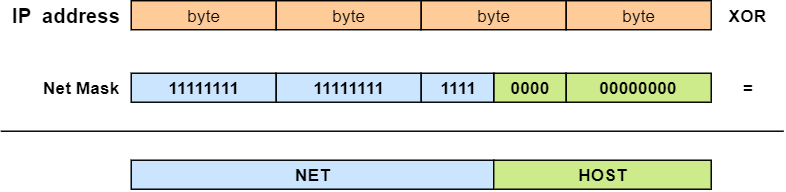
\includegraphics[scale=0.5]{Images/IP/netmask}
\caption{\footnotesize{Example of netmask use.}}\label{netmask}
\end{figure}
\begin{figure}[h]
\centering
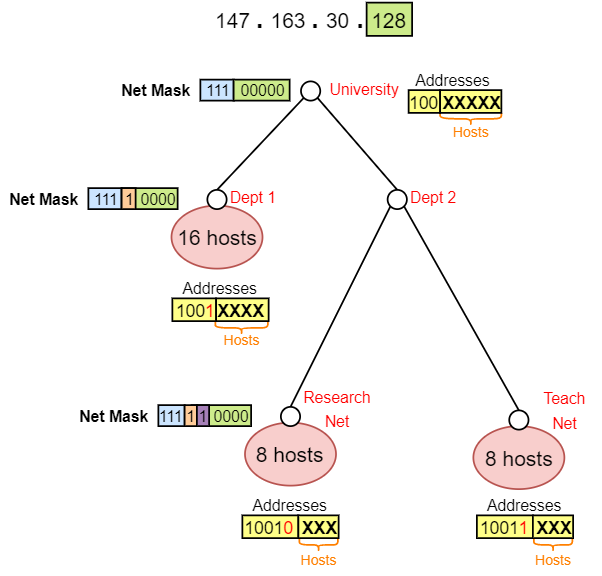
\includegraphics[scale=0.55]{Images/IP/dei_IP}
\caption{\footnotesize{Example of subnetworks structure.}}\label{dei_ip}
\end{figure}
\begin{figure}[h]
\centering
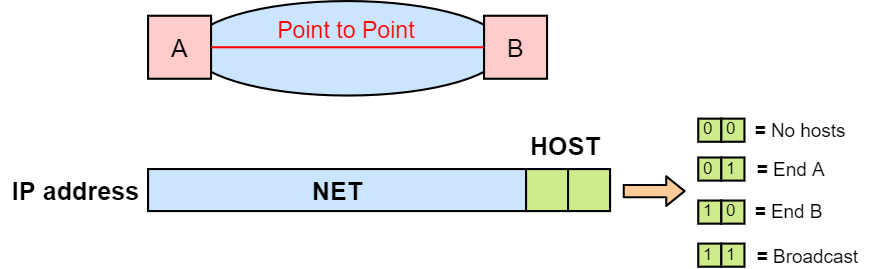
\includegraphics[scale=0.4]{Images/IP/point2point}
\caption{\footnotesize{Example of Point to Point connection network.}}\label{point2point}
\end{figure}
\clearpage
\section{Fragmentation}\label{fragment_section}
In each network, the IP information is embedded in a Layer 3 packet that respects protocol of the network in which it is. Then when the packet reach a gateway, its IP info is removed from the packet and encapsulated in a Layer 2 packet, to be sent to another network (Figure \ref{packets}). Each IP packet is also called \textbf{Datagram}.\\
Each network is defined by a Maximum Transfer Unit (MTU), that defines the maximum size of each Layer 3 packet inside the network. Hence, if the IP information, that reach a gateway of the network, is larger than MTU, the gateway reduces its size (Figure \ref{fragmentation}).\\
If a packet pass through many networks and their MTUs are very different, using datagrams, we are sure that the packets won't arrive as in the same order in which they are sent. The reason why this happens is that they are sent without the use of a stream. To manage this problem, when the gateway creates a packet, this stores the first index of the sequence of the bytes of the original IP information.\\
The last packet, that composed initial IP message, has the flag \textbf{More Fragments(MF)} set to 0. This information with the knowledge of the length and the first byte index of the last packet, permits to define the length of the original message, whenever it arrives. Each packet can fit easly in the buffer of the gateway receiver (Figure \ref{label_fragment}).
\begin{figure}[h]
\centering
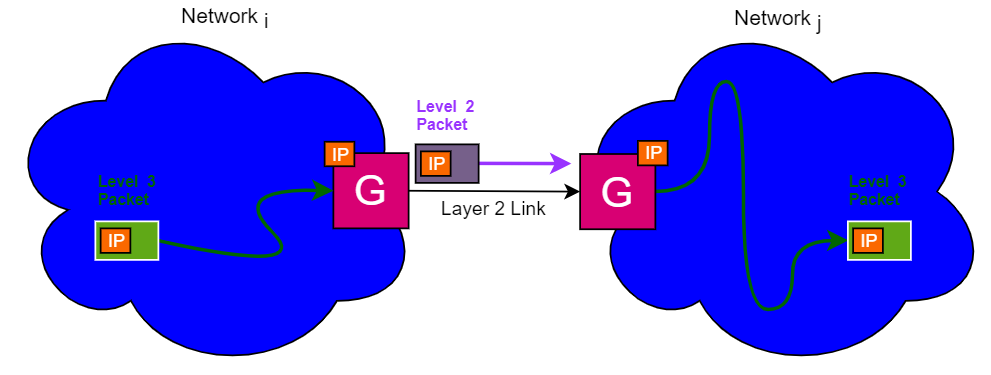
\includegraphics[scale=0.5]{Images/IP/packets}
\caption{\footnotesize{Example of encapsulation of IP packet.}}\label{packets}
\end{figure}
\begin{figure}[h]
\centering
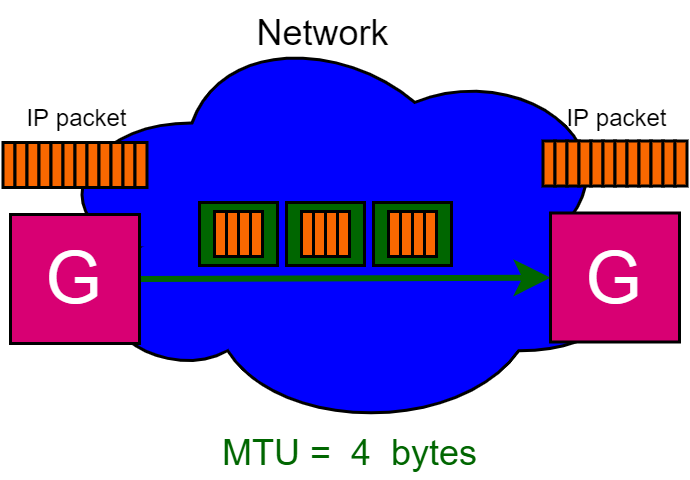
\includegraphics[scale=0.4]{Images/IP/fragmentation}
\caption{\footnotesize{Example of fragmentation.}}\label{fragmentation}
\end{figure}
\begin{figure}[h]
\centering
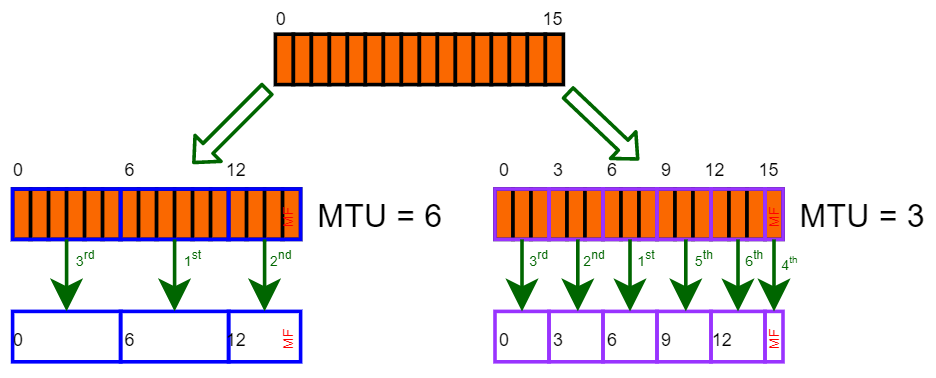
\includegraphics[scale=0.4]{Images/IP/label_fragment}
\caption{\footnotesize{Example of fragment labeling.}}\label{label_fragment}
\end{figure}

\section{Internet Header Format}
\begin{figure}[h]
\centering
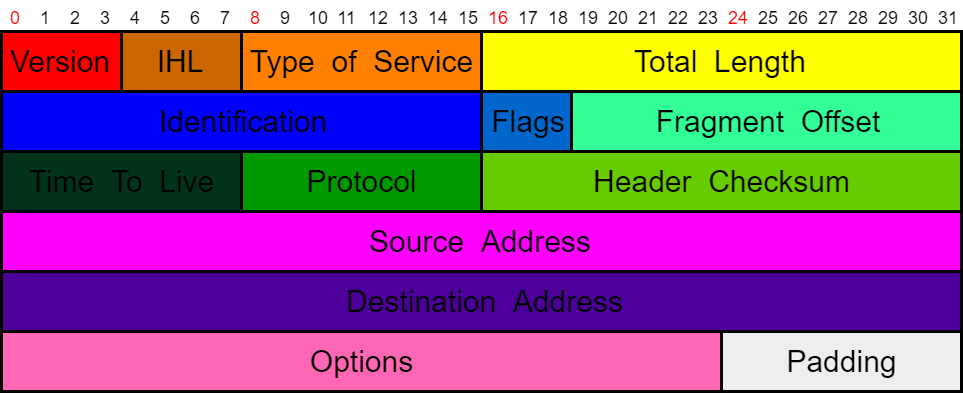
\includegraphics[scale=0.3]{Images/IP/internet_header}
\caption{\footnotesize{Internet header format.}}\label{internet_header}
\end{figure}
The content of the internet header is (Figure \ref{internet_header}):
\begin{itemize}
\item{\textbf{Version}
format of the internet header
}
\item{\textbf{IHL}\\
length, measured in words of 32 bits, of the internet header (minimum value = 5)
}
\item{\textbf{Type of Service}\\
parameters of the Quality of Service (QoS) desired (Figure \ref{flags}). Bits \textbf{6-7} are reserved for future use.
\begin{figure}[h]
\centering
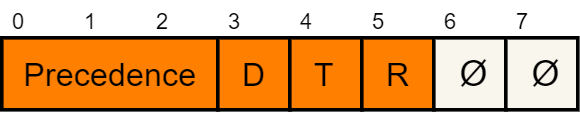
\includegraphics[scale=0.3]{Images/IP/service_type}
\caption{\footnotesize{Type of service field.}}\label{service_type}
\end{figure}
\begin{table}[h]
\centering \footnotesize
\begin{tabular}{|c|c|c|c|}
\cline{2-4}
\multicolumn{1}{c|}{}&{Delay (D)}&{Throughput(T)}&{Relaibility (R)}\\
\hline
{0}&{Normal}&{Normal}&{Normal}\\
\hline
{1}&{Low}&{High}&{High}\\
\hline
\end{tabular}
\caption{Bits 3,4,5 of Type of Service.}
\end{table}
\begin{table}[H]
\centering \footnotesize
\begin{tabular}{|c|l|}
\hline
\textbf{111}&{Network Control}\\
\hline
\textbf{110}&{Internetwork Control}\\
\hline
\textbf{101}&{CRITIC/ECP}\\
\hline
\textbf{100}&{Flash Override}\\
\hline
\textbf{011}&{Flash}\\
\hline
\textbf{010}&{Immediate}\\
\hline
\textbf{001}&{Priority}\\
\hline
\textbf{000}&{Routine}\\
\hline
\end{tabular}
\caption{Precedence of Type of Service.}
\end{table}
}
\item{\textbf{Total Length}\\
length, measured in octets, including internet header and data.\\
This field allows the length of a datagram to be up to 65,535 octets. Such long datagrams are impractical for most hosts and networks.  All hosts must be prepared to accept datagrams of up to 576 octets (whether they arrive whole or in fragments).  It is recommended that hosts only send datagrams larger than 576 octets if they have assurance that the destination is prepared to accept the larger datagrams.
}
\item{\textbf{Identification}\\
an identifying value assigned by the sender to aid in assembling the fragments of a datagram.\\
It's a random number generated by host while creating the packet, that is different from numbers of all other packets.
}
\item{\textbf{Flags}\\
varius control flags. The bit 0 is reserved and must be 0.
\begin{figure}[h]
\centering
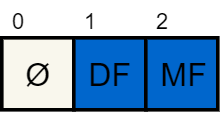
\includegraphics[scale=0.3]{Images/IP/flags}
\caption{\footnotesize{Flags.}}\label{flags}
\end{figure}
\begin{table}[H]
\centering \footnotesize
\begin{tabular}{|c|c|c|}
\cline{2-3}
\multicolumn{1}{c|}{}&{Don't Fragment (DF)}&{More Fragments (MF)}\\
\hline
{0}&{May Fragment}&{Last Fragment}\\
\hline
{0}&{Don't Fragment}&{More Fragments}\\
\hline
\end{tabular}
\caption{DF and MF flags.}
\end{table}
If DF set and a packet that arrives to a network should be divided in smaller fragments, it's dropped.
}
\item{\textbf{Fragment Offset}\\
This field indicates where in the datagram this fragment belongs (position of the fragment in the original long packet).\\
The fragment offset is measured in units of 8 octets (64 bits).  The first fragment has offset zero.\\ It's computed starting from initial position in the packet.
}
\item{\textbf{Time to Live}\\
maximum time (number of forward for the packet) the datagram is allowed to remain in the internet system.\\
This counter is set by host that generated the packet. Every node in the network (routers, switches), that process the packet, decrements the value of this field.\\
When a node, decrementing this field, reaches zero value for Time To Live, it drops the packet immediately.\\
Time To Live prevents that a packet stays in the network too much time compromising infrustructure efficiency.
}
\item{\textbf{Protocol}\\
the next level protocol (Layer 4) used in the data portion of the internet datagram. In general it's called ULP (Upper Layer Protocol). This is useful and was done also at upper layer, using port numbers, because it's a way to communicate future use to upper layer. This field is the upper layer protocol type (\textbf{/etc/protocols} on UNIX) and it's used by Operating System to understand to which module send a specific part of the packet. You can also find them in IANA site\cite{IANA_IP_protocol}.
}
\item{\textbf{Header Checksum}\\
a checksum on the header only.\\\\
\textit{How to compute it}\\
The checksum field is the 16 bit one's complement of the one's complement sum of all 16 bit words in the header.  For purposes of computing the checksum, the value of the checksum field is zero. The two main operation used in its computation are:
\begin{itemize}
\item{\textbf{One's complement sum(}$\oplus$\textbf{)}\\
two words of 16 bits are summed up, bit by bit, and the last carry is summed up to the previous result. The following example shows how to sum two number with this operator:
\begin{table}[h]
\centering\footnotesize
\begin{tabular}{rl}
{10110 ... 10} & {\textbf{+}}\\
{01101 ... 11} & {\textbf{=}}\\
\hline
{00100 ... 01} & {\textbf{+}}\\
{carry: 1} & {\textbf{=}}\\
\hline
{00100 ... 10} &\\
\end{tabular}
\end{table}
}

\item{\textbf{Ons's complement}\\
the value of each bit, inside the result of 16 bit sum of all the words, change their values.
\begin{table}[h]
\centering\footnotesize
\begin{tabular}{r}
{00100 ... 10} \\
\hline
{11011 ... 01} \\
\end{tabular}
\end{table}
}
\end{itemize}
\begin{figure}[h]
\centering
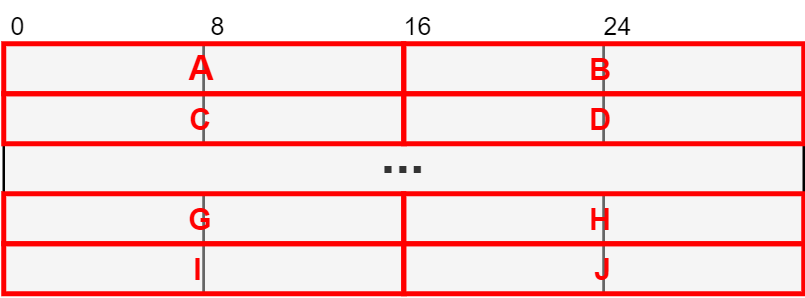
\includegraphics[scale=0.3]{Images/IP/checksum}
\caption{\footnotesize{Words of payload evaluated in checksum.}}\label{checksum}
\end{figure}
$$Checksum\;=\;\textasciitilde(A\oplus B \oplus C\oplus D\oplus ...\oplus A\oplus B \oplus C\oplus D\oplus)$$
This algorithm is very simple but experimental evidence indicates it works. Nowadays, it's quite always used CRC procedure.
}
\item{\textbf{Source Address}\\
the source IP address
}
\item{\textbf{Destination Address}\\
the destination IP address
}
\item{\textbf{Options}\\
it'svariable and it may appear or not in datagrams. They must be implemented by all IP modules (host and gateways).\\
What is optional is their transmission in any particular datagram, not their implementation.
}
\end{itemize}
\chapter{HTTP protocol}
HTTP protocol was presented for the first time in the RFC 1945 (Request for Comment).\\
The Hypertext Transfer Protocol (HTTP) is an application-level protocol with the lightness and speed necessary for distributed, collaborative, hypermedia information systems. It is a generic, stateless, object-oriented protocol which can be used for many tasks, such as name servers and distributed object management systems, through extension of its request methods (commands).\\
It's not the first Hypertext protocol in history because there was Hypertalk, made by Apple before. \\
A feature of HTTP is the typing of data representation, allowing systems to be built independently f the data being transferred. HTTP has been in use by the World-Wide Web global information initiative since 1990.

\section{Terminology}
\begin{itemize}
\item{\textbf{connection}\\
a transport layer virtual circuit established between two application programs for the purpose of communication.}
\item{\textbf{message}\\
the basic unit of HTTP communication, consisting of a structured sequence of octets matching the syntax defined in Section 4 and transmitted via the connection.}
\item{\textbf{request}\\
an HTTP request message.
}
\item{\textbf{response}\\
an HTTP response message.}
\item{\textbf{resource}\\
a network data object or service which can be identified by a URI.}
\item{\textbf{entity}\\
a particular representation or rendition of a data resource, or reply from a service resource, that may be enclosed within a request or response message. An entity consists of metainformation in the form of entity headers and content in the form of an entity body.}
\item{\textbf{client}\\
an application program that establishes connections for the purpose of sending requests.}
\item{\textbf{user agent}\\
the client which initiates a request. These are often browsers, editors, spiders (web-traversing robots), or other end user tools.}
\item{\textbf{server}\\
an application program that accepts connections in order to service requests by sending back responses.}
\item{\textbf{origin server}\\
the server on which a given resource resides or is to be created.}
\item{\textbf{proxy}\\
an intermediary program which acts as both a server and a client for the purpose of making requests on behalf of other clients. Requests are serviced internally or by passing them, with possible translation, on to other servers. A proxy must interpret and, if necessary, rewrite a request message before forwarding it.\\
Proxies are often used as client-side portals
through network firewalls and as helper applications for handling requests via protocols not implemented by the user agent.}
\item{\textbf{gateway}\\
a server which acts as an intermediary for some other server. Unlike a proxy, a gateway receives requests as if it were the origin server for the requested resource; the requesting client may not be aware that it is communicating with a gateway.\\
Gateways are often used as server-side portals through network firewalls and as protocol translators for access to resources stored on non-HTTP systems.}
\item{\textbf{tunnel}\\
a tunnel is an intermediary program which is acting as a blind relay between two connections. Once active, a tunnel is not considered a party to the HTTP communication, though the tunnel may have been initiated by an HTTP request. The tunnel ceases to exist when both ends of the relayed connections are closed.\\
Tunnels are used when a portal is necessary and the intermediary cannot, or should not, interpret the relayed communication.}
\item{\textbf{cache}\\
a program's local store of response messages and the subsystem that controls its message storage, retrieval, and deletion. A cache stores cachable responses in order to reduce the response time and network bandwidth consumption on future, equivalent requests. Any client or server may include a cache, though a cache cannot be used by a server while it is acting as a tunnel.}
\end{itemize}
Any given program may be capable of being both a client and a server; our use of these terms refers only to the role being performed by the program for a particular connection, rather than to the program's capabilities in general. Likewise, any server may act as an origin server, proxy, gateway, or tunnel, switching behavior based on the nature of each request.

\section{Basic rules}
The following rules are used throughout are used to describe the grammar used in the RFC 1945.
\begin{table}[h]
\centering
\footnotesize
\begin{tabular}{rl}
\textbf{OCTET =}& <any 8-bit sequence of data>\\
\textbf{CHAR =}& <any US-ASCII character (octets 0 - 127)>\\
\textbf{UPALPHA =}& <any US-ASCII uppercase letter "A".."Z">\\
\textbf{LOALPHA =}& <any US-ASCII lowercase letter "a".."z">\\
\textbf{ALPHA =}& UPALPHA | LOALPHA\\
\textbf{DIGIT =}& <any US-ASCII digit "0".."9">\\
\textbf{CTL =}& <any US-ASCII control character (octets 0 - 31) and DEL (127)>\\
\textbf{CR =}& <US-ASCII CR, carriage return (13)>\\
\textbf{LF =}& <US-ASCII LF, linefeed (10)>\\
\textbf{SP =}& <US-ASCII SP, space (32)>\\
\textbf{HT =}& <US-ASCII HT, horizontal-tab (9)>\\
\textbf{<"> =}& <US-ASCII double-quote mark (34)>\\
\end{tabular}
\end{table}

\section{Messages}
\subsection{Different versions of HTTP protocol}
\begin{itemize}
\item{\textbf{HTTP/0.9 Messages}\\
Simple-Request and Simple-Response do not allow the use of any header information and are limited to a single request method (GET).\\ Use of the Simple-Request format is discouraged because it prevents the server from identifying the media type of the returned entity.
\begin{center}
\begin{tabular}{c}
\begin{lstlisting}[linewidth=240pt, basicstyle=\footnotesize\sffamily,]
HTTP-message = Simple-Request | Simple-Response
\end{lstlisting}
\end{tabular}
\end{center}
\begin{center}
\begin{tabular}{c}
\begin{lstlisting}[linewidth=230pt, basicstyle=\footnotesize\sffamily,]
Simple-Request  = "GET" SP Request-URI CRLF


Simple-Response = [ Entity-Body ]
\end{lstlisting}
\end{tabular}
\end{center}
}
\item{\textbf{HTTP/1.0 Messages}\\
Full-Request and Full-Response use the generic message format of RFC 822 for transferring entities. Both messages may include optional header fields (also known as "headers") and an entity body. The entity body is separated from the headers by a null line (i.e., a line with nothing preceding the CRLF).
\begin{center}
\begin{tabular}{c}
\begin{lstlisting}[linewidth=230pt, basicstyle=\footnotesize\sffamily,]
HTTP-message = Full-Request | Full-Response
\end{lstlisting}
\end{tabular}
\end{center}
\begin{center}
\begin{tabular}{c}
\begin{lstlisting}[linewidth=340pt, basicstyle=\footnotesize\sffamily,]
Full-Request = Request-Line
               *(General-Header | Request-Header | Entity-Header)
               CRLF
               [Entity-Body]
               
               
Full-Response = Status-Line
                *(General-Header | Request-Header | Entity-Header)
                CRLF
                [Entity-Body]               
\end{lstlisting}
\end{tabular}
\end{center}
}
\end{itemize}

\subsection{Headers}
The order in which header fields are received is not significant. However, it is "good practice" to send General-Header fields first, followed by Request-Header or Response-Header fields prior to the Entity-Header fields.\\
Multiple HTTP-header fields with the same field-name may be present in a message if and only if the entire field-value for that header field is defined as a comma-separated list.
\begin{center}
\begin{tabular}{c}
\begin{lstlisting}[linewidth=260pt, basicstyle=\footnotesize\sffamily,]
HTTP-header = field-name ":" [ field-value ] CRLF
\end{lstlisting}
\end{tabular}
\end{center}

\subsection{Request-Line}
\begin{center}
\begin{tabular}{c}
\begin{lstlisting}[linewidth=320pt, basicstyle=\footnotesize\sffamily,]
Request-Line = Method SP Request-URI SP HTTP-Version CRLF

Method         = "GET" | "HEAD" | "POST" | extension-method

extension-method = token
\end{lstlisting}
\end{tabular}
\end{center}
The list of methods acceptable by a specific resource can change dynamically; the client is notified through the return code of the response if a method is not allowed on a resource.\\
Servers should return the status code 501 (not implemented) if the method is unrecognized or not implemented.

\subsection{Request-URI}
The Request-URI is a Uniform Resource Identifier and identifies the resource upon which to apply the request.
\begin{center}
\begin{tabular}{c}
\begin{lstlisting}[linewidth=190pt, basicstyle=\footnotesize\sffamily,]
Request-URI = absoluteURI | abs_path
\end{lstlisting}
\end{tabular}
\end{center}
The absoluteURI form is only allowed when the request is being made to a proxy. The proxy is requested to forward the request and return the response. If the request is GET or HEAD and a prior response is cached, the proxy may use the cached message if it passes any restrictions in the Expires header field.\\
Note that the proxy may forward the request on to another proxy or directly to the server specified by the absoluteURI. In order to avoid request loops, a proxy must be able to recognize all of its server names, including any aliases, local variations, and the numeric IP address.\\\\
The most common form of Request-URI is that used to identify a resource on an origin server or gateway. In this case, only the absolute path of the URI is transmitted.

\subsection{Request Header}
The request header fields allow the client to pass additional information about the request, and about the client itself, to the server.\\
These fields act as request modifiers, with semantics equivalent to the parameters on a programming language method (procedure) invocation.
\begin{center}
\begin{tabular}{c}
\begin{lstlisting}[linewidth=410pt, basicstyle=\footnotesize\sffamily,]
Request-Header = Authorization | From | If-Modified-Since | Referer | User-Agent
\end{lstlisting}
\end{tabular}
\end{center} 

\subsection{Status line}
\begin{center}
\begin{tabular}{c}
\begin{lstlisting}[linewidth=330pt, basicstyle=\footnotesize\sffamily,]
Status-Line = HTTP-Version SP Status-Code SP Reason-Phrase CRLF
\end{lstlisting}
\end{tabular}
\end{center}
\begin{table}[h]
\centering
\footnotesize
\begin{tabular}{|r|l|}
\multicolumn{2}{c}{\textbf{General Status code}}\\
\hline
\textbf{1xx: Informational} & {Not used, but reserved for future use}\\
\hline
\textbf{2xx: Success}&{The action was successfully received,}\\
\hline
& {understood, and accepted.}\\
\hline
\textbf{3xx: Redirection} & {Further action must be taken in order to}\\
&{complete the request}\\
\hline
\textbf{4xx: Client Error}&{The request contains bad syntax or cannot}\\
&{be fulfilled}\\
\hline
\textbf{5xx: Server Error}&{The server failed to fulfill an apparently}\\
&{valid request}\\
\hline
\end{tabular}
\end{table}
\begin{table}[h]
\centering
\footnotesize
\begin{tabular}{|r|l|}
\multicolumn{2}{c}{\textbf{Known service code}}\\
\hline
\textbf{200}&{OK}\\
\hline
\textbf{201}&{Created}\\
\hline
\textbf{202}&{Accepted}\\
\hline
\textbf{204}&{No Content}\\
\hline
\textbf{301}&{Moved Permanently}\\
\hline
\textbf{302}&{Moved Temporarily}\\
\hline
\textbf{304}&{Not Modified}\\
\hline
\textbf{400}&{Bad Request}\\
\hline
\textbf{401}&{Unauthorized}\\
\hline
\textbf{403}&{Forbidden}\\
\hline
\textbf{404}&{Not Found}\\
\hline
\textbf{500}&{Internal Server Error}\\
\hline
\textbf{501}&{Not Implemented}\\
\hline
\textbf{502}&{Bad Gateway}\\
\hline
\textbf{503}&{Service Unavailable}\\
\hline
\end{tabular}
\end{table}

\vspace{10cm}
\section{Examples}
The following pieces of code are examples of TCP client connection to \textbf{www.google.it}, using functions explained in Chapter \ref{networkC}.
\subsection{HTTP 0.9}
The following piece of code define a structure, used to connect to Google server. 

The most important thing is that \textbf{socket()} is entry-point for level 4, but also \textbf{connect()} is the request to Kernel to extablish the connection.\\ \textbf{read()} and \textbf{write()} are system calls used respectively to obtain result(response) of a request and to generate request.\\ These function permit us to ask to lower level to do this things, without knowing content of system buffers (stream). The second part is only used to read the input.

\subsection{HTTP 1.0}
The protocol has no mandatory headers to be added in the request field. This protocol is compliant with HTTP 0.9.
To keep the connection alive, "Connection" header with "keep-alive" as header field must be added to request message. The server, receiving the request, replies with a message with the same header value for "Connection".\\
This is used to prevent the closure of the connection, so if the client needs to send another request, he can use the same connection.
This is usually used to send many files and not only one.\\
The connection is kept alive until either the client or the server decides that the connection is over and one of them drops the connection. If the client doesn't send new requests to the server, the second one usually drops the connection after a couple of minutes.\\
The client could read the response of request, with activated keep alive option, reading only header and looking to "Content-length" header field value to understand the length of the message body. This header is added only if a request with keep-alive option is done.\\
This must be done because we can't look only to empty system stream, because it could be that was send only the response of the first request or a part of the response.\\
Otherwise, when the option keep alive is not used, the client must fix a max number of characters to read from the specific response to his request, because he doesn't know how many character compose the message body. If you make many requests to server without keep-alive option, the server will reply requests, after the first, with only headers but empty body.\\

\subsection{HTTP 1.1}
It has by default the option keep alive actived by default with respect to HTTP 1.0. It has the mandatory header "Host" followed by the hostname of the remote system to which the request or the response is sent. The body is organized in chunks, so we need the connection kept alive to manage future new chunks.\\
This is useful with dynamic pages, in which the server doesn't know the length of the stream in advance and can update the content of the stream during the extablished connection, sending a fixed amount of bytes to client. We can check if the connection is chunked oriented, looking for the header "Transfer-Encoding" with value "chunked".\\ 
Each connection is composed by many chunks and each of them is composed by chunk length followed by chunk body, except for the last one that has length 0 (see Figure \ref{chunked_body}). The following grammar represents how the body is organized:
\begin{center}
\begin{tabular}{c}
\begin{lstlisting}[linewidth=320pt, basicstyle=\footnotesize\sffamily,]
Chunked-Body   = *chunk
                 last-chunk
                 trailer
                 CRLF

chunk          = chunk-size [ chunk-extension ] CRLF
                 chunk-data CRLF

chunk-size     = 1*HEX
last-chunk     = 1*("0") [ chunk-extension ] CRLF

chunk-extension= *( ";" chunk-ext-name [ "=" chunk-ext-val ] )

chunk-ext-name = token
chunk-ext-val  = token | quoted-string
chunk-data     = chunk-size(OCTET)
trailer        = *(entity-header CRLF)
\end{lstlisting}
\end{tabular}
\end{center}

\begin{figure}[h]
\centering
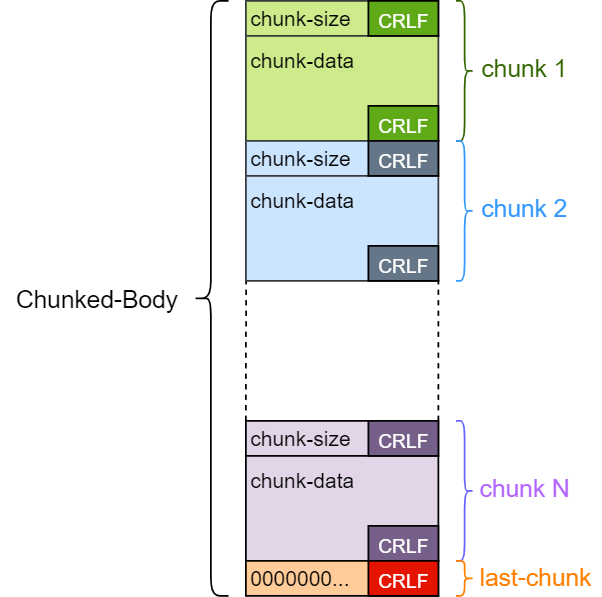
\includegraphics[scale=0.5]{Images/HTTP/Chunked-Body}\caption{\footnotesize{Chunked body.}}\label{chunked_body}
\end{figure}

\section{HTML}
The body of an HTTP request, it's often composed from the HTML related page. Each click, of a link inside the web page, generates a new request to the server with GET method.
\chapter{Resolution of names}
The following section will talk about history of technologies under the resolution of server names in URL to their IP addresses, needed to extablish the connection.

\section{Network Information Center (NIC)}\label{NIC_section}
This type of architecture was used in the past to resolve names. Each client has its own file \textbf{HOSTS.txt}, with resolution of names. The client shared its file with a central system, called \textbf{NIC} (Figure \ref{NIC}). This system collects all the files, like an hub, and shared resolution names to other clients.\\
This architecture is unfeasable and not scalable with nowadays number of IP addresses, because the files become very huge and transfering becomes very slow.\\
\begin{figure}[h]
\centering
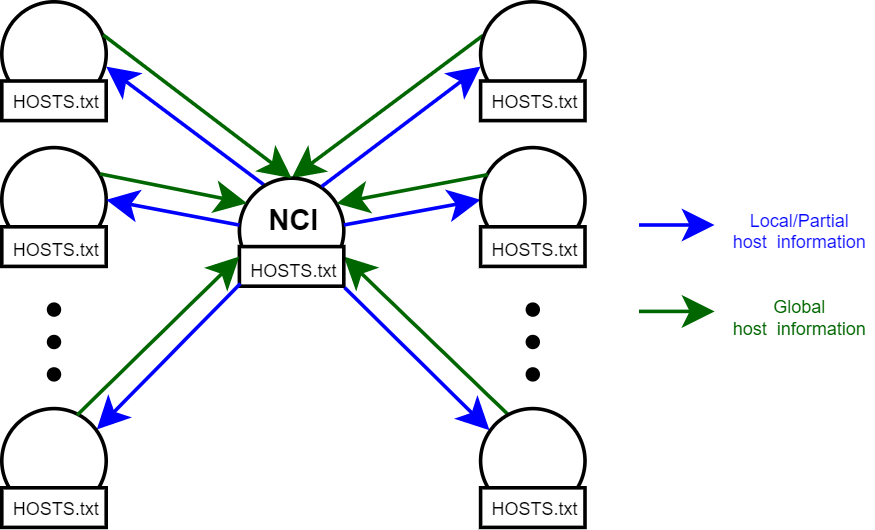
\includegraphics[scale=0.4]{Images/Resolution/NIC}
\caption{\footnotesize{How NIC worked.}}\label{NIC}
\end{figure}


\section{Domain Name System (DNS)}\label{DNS_system}
The file \textbf{HOSTS.txt} is yet used in nowadays UNIX systems (Section \ref{NIC_section}). The specified host name is searched in local \textbf{/etc/hosts.txt}, that contains local and private addresses resolution table, and if not found, it will be searched through DNS\cite{RFC1034}.

\subsection{Goals}
\begin{enumerate}
\item{Names should not be required to contain network identifiers, addresses, routes, or similar information as part of the name.}
\item{The sheer size of the database and frequency of updates suggest that it must be maintained in a distributed manner, with local caching to improve performance.\\
Approaches that attempt to collect a consistent copy of the entire database will become more and more expensive and difficult, and hence should be avoided.\\
The same principle holds for the structure of the name space, and in particular mechanisms for creating and deleting names; these should also be distributed.}
\item{Where there are tradeoffs between the cost of acquiring data, the speed of updates, and the accuracy of caches, the source of the data should control the tradeoff.}
\item{The costs of implementing such a facility dictate that it be generally useful, and not restricted to a single application.\\
We should be able to use names to retrieve host addresses, mailbox data, and other as yet undetermined information. All data associated with a name is tagged with a type, and queries can be limited to a single type.}
\item{Because we want the name space to be useful in dissimilar networks and applications, we provide the ability to use the same name space with different protocol families or management.\\
For example, host address formats differ between protocols, though all protocols have the notion of address. The DNS tags all data with a class as well as the type, so that we can allow parallel use of different formats for data of type address.}
\item{We want name server transactions to be independent of the communications system that carries them.\\
Some systems may wish to use datagrams for queries and responses and only establish virtual circuits for transactions that need the reliability (e.g., database updates, long transactions); other systems will use virtual circuits exclusively.}
\item{The system should be useful across a wide spectrum of host capabilities.\\
Both personal computers and large timeshared hosts should be able to use the system, though perhaps in different ways.}
\end{enumerate}

\subsection{Hierarchy structure}
Hierarchy permits to manage a lot of nambers of domain names and IP addresses, reducing the time spent to resolve them. Given for example the host name \textbf{www.dei.unipd.it}, we have a \textbf{Name Server (NS)} for each of the domain name inside it (Figure \ref{DNS_hierarchy}). The tree hierarchy has a name server for each one of its internal nodes.The name server gives us only the name of the name server of the lower level to which we need to go.\\
To obtain the IP address of this name server, we need to ask, to name server of upper layer, a \textbf{glue record}. The glue record is an additional information that is needed by us to understand how to reach that name server. Hence the glue record is the IP address of NS of the lower level in hierarchy. \\
For each request to NS, we obtain also the expiration time information because a caching approach is adopted in DNS but at level 4. There are 13 root name servers that are obtained when asking resolution to root. \\
In reality root name servers are more than 13 but the communication used in DNS is made through UDP and this type of connection supports only 13 simultaneously transfers. The local DNS server for the device, managed by my network provider, contains the 13 root servers and permits us to reach at least one DNS root server.\\
The 13 DNS root servers are added locally during the installation of local DNSs and updated assuming that at least one root server of them can be reachable. There is no address record for the root.\\
In general structure of the queries to name servers, we ask only the resolution for a specific domain that composes the whole name (Figure \ref{default_DNS}).\\
To use a caching system efficiently, we need to make a recursive query, sending the request of resolution of the whole name with all its domains (Figure \ref{recursive_DNS}). All the name servers, where the query passes throuh, store information about resolution. This system is never applied as it is.\\
In reality an hybrid version is implemented, using only partial recursion (Figure \ref{hybrid_DNS}). Local DNS usually has huge cache with main important names and also first and second level have caches. So local DNS rarely asks resolution to TOP Level Domain or Root.\\
Recursive query option in dig command is made by a flag, default set to yes and used in UDP packet as an additional information. The Root Name Server decides if it wants to accept recursive query or if not, how many domains can resolve. I can group some domains, defining a zone, so I can use only a name server for a specific zone to solve many domains together (Figure \ref{DNS_zone}). So the name servers are authorithative over zones and not only single domains.\\
The creation of the zones are used to manage easily the responsability of companies and their organization over the zones, grouping domains. Another reason for this partition in zones is the presence of some domains with few names, that it's better to group with other domains.
\begin{figure}[h]
\centering
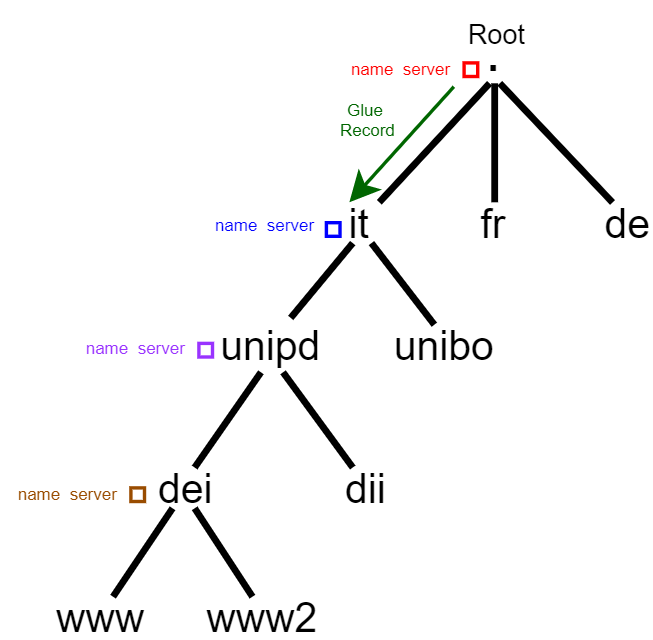
\includegraphics[scale=0.38]{Images/Resolution/DNS_hierarchy}
\caption{\footnotesize{DNS structure.}}\label{DNS_hierarchy}
\end{figure}
\begin{lstlisting}[linewidth=470pt, style=code, caption=Example of default DNS queries using dig.]
//Ask for root name server to the default name server 
dig -t NS -n .
 
//Ask for address of root name server "a.root-servers.net", previously chosen
dig -t A -n a.root-servers.net 

//Ask for "it" name server to the "a.root-servers.net" address, previously chosen
dig @198.41.0.4 -t NS it 

//Ask for address of "nameserver.cnr.it" name server,  previously chosen for "it" domain
dig @198.41.0.4 -t A  nameserver.cnr.it

//Ask for "unipd.it" name server to the "nameserver.cnr.it" address 
dig @194.119.192.34 -t NS -n unipd.it

//Ask for "unipd.it" name server to the "nameserver.cnr.it" address 
dig @194.119.192.34 -t A unipd.it

//Ask for "dei.unipd.it" name server to one ("mail.dei.unipd.it" 
dig @147.162.1.100 -t NS  dei.unipd.it

//Ask for address of "mail.dei.unipd.it" name server, previously chosen 
dig @147.162.1.2 -t A  mail.dei.unipd.it 

//Ask for address of "www.dei.unipd.it" to "mail.dei.unpd.it" name server, previousy chosen 
dig @147.162.2.100 -t A  www.dei.unipd.it
\end{lstlisting} 
\begin{figure}[h]
\centering
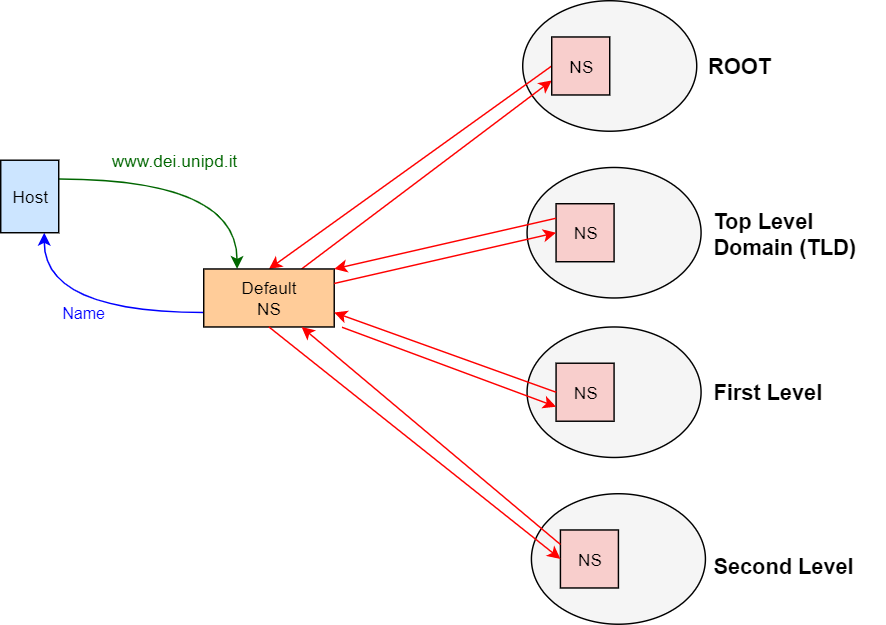
\includegraphics[scale=0.4]{Images/Resolution/default_DNS}
\caption{\footnotesize{Default DNS behaviour without caching.}}\label{default_DNS}
\end{figure}
\begin{figure}[h]
\centering
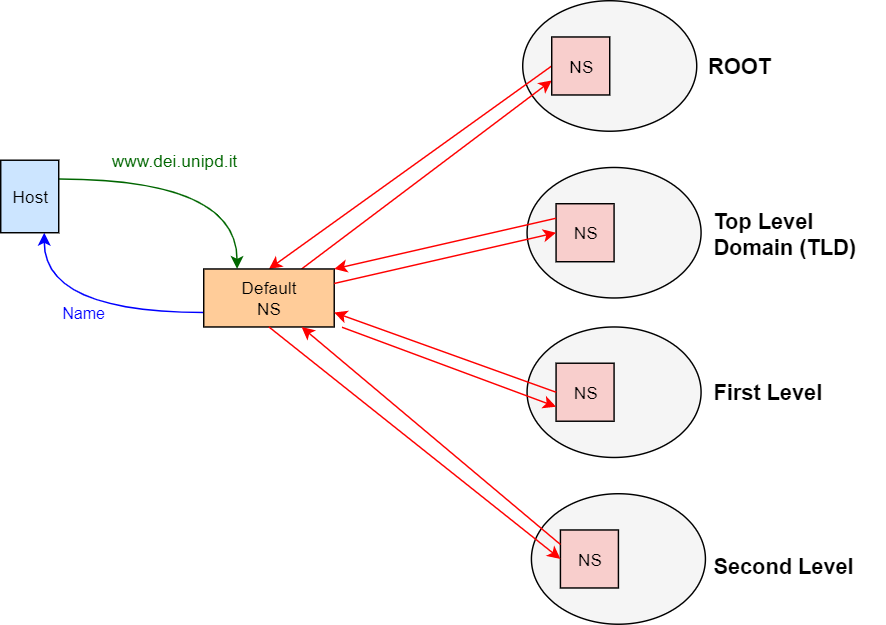
\includegraphics[scale=0.4]{Images/Resolution/default_DNS}
\caption{\footnotesize{Completely recursive DNS structure.}}\label{recursive_DNS}
\end{figure}
\begin{figure}[h]
\centering
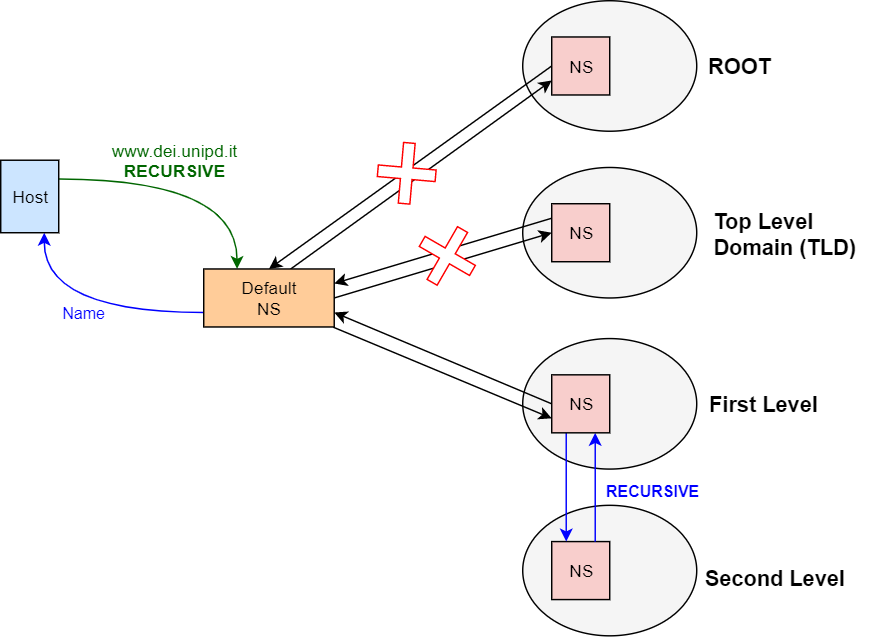
\includegraphics[scale=0.4]{Images/Resolution/hybrid_DNS}
\caption{\footnotesize{Hybrid DNS structure.}}\label{hybrid_DNS}
\end{figure}
\begin{figure}[H]
\centering
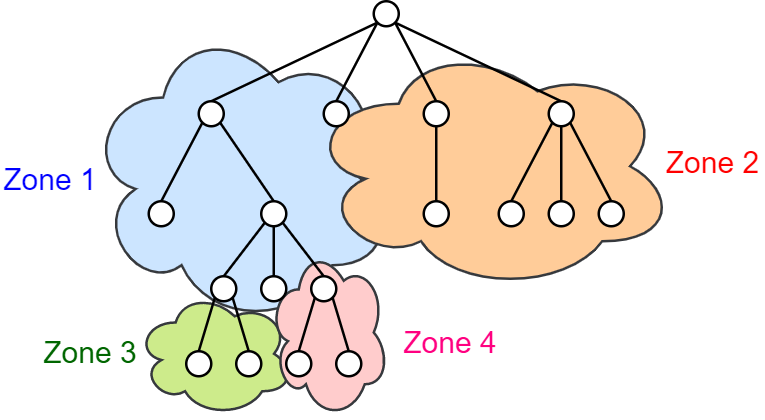
\includegraphics[scale=0.4]{Images/Resolution/DNS_zone}
\caption{\footnotesize{Example of partitioning into zones.}}\label{DNS_zone}
\end{figure}
\begin{comment}
\chapter{HTML}
The body of an HTTP request, it's often composed from the HTML related page. Each click, of a link inside the web page, generates a new request to the server with GET method.
\chapter{CSS}
\chapter{Javascript}
\chapter{PHP}
\end{comment}
\chapter{Shell}

\section{Commands}

\begin{table}[h]
\centering
\footnotesize
\begin{tabular}{|l|l|l|}
\hline
\multicolumn{2}{|l|}{\multirow{2}{*}{\textbf{man} man}}&{Shows info about man command and}\\
\multicolumn{2}{|l|}{} & {lists all the sections of the manual.}\\
\hline
\multicolumn{2}{|l|}{\textbf{strace} objFile} & {Lists all the system calls used in the program.}\\
\hline
\multicolumn{2}{|l|}{\textbf{gcc} -o objFile source \textbf{-v}} & {Lists all the path of libraries and headers used in creation of objFile.}\\
\hline
\multirow{3}{*}{\textbf{netstat}} & {-t} & {Lists all the active TCP connections showing domain names.}\\
\cline{2-3}
& {-u} & {Lists all the active UDP connections showing domain names.}\\
\cline{2-3}
& {-n} & {Lists all the active, showing IP and port numbers.}\\
\hline
\multicolumn{2}{|l|}{\textbf{nslookup} domain} & {Shows the IP address related to the domain (E.g. IP of www.google.it)}\\
\hline
\multicolumn{2}{|l|}{\multirow{5}{*}{\textbf{dig} @server name type}}&{DNS lookup utility.}\\
\multicolumn{2}{|l|}{}&{\textbf{server} name or IP address of the name server to query}\\
\multicolumn{2}{|l|}{}&{\textbf{name} name of the resource record that is to be looked up}\\
\multicolumn{2}{|l|}{}&{\textbf{type} type of query is required (ANY, A, MX, SIG, etc.)}\\
\multicolumn{2}{|l|}{}&{$\;\;\;\;\;\;\;\;\;\;$if no type is specified, A is performed by default}\\
\hline
\multicolumn{2}{|l|}{\multirow{2}{*}{\textbf{wc} [file]}} & {Prints in order newlines, words, and bytes (characters) counts for file}\\
\multicolumn{2}{|l|}{} & {if file not specified or equal to -, counts from stdin.}\\
\hline
\multicolumn{2}{|l|}{\multirow{2}{*}{\textbf{route} -n}} & {Show numerical addresses instead of trying to determine symbolic}\\
\multicolumn{2}{|l|}{} & {hostnames in routing table.}\\
\hline
\end{tabular}
\end{table}


\section{UNIX Files}\label{files}
\begin{table}[h]
\centering
\footnotesize
\begin{tabular}{|l|l|}
\hline
\textbf{/etc/hosts} & {Local resolution table.}\\
\hline
\multirow{2}{*}{\textbf{/etc/services}} & {List all the applications with their port}\\
& {and type of protocol (TCP/UDP).}\\
\hline
{\textbf{/etc/protocols}} & {Internet protocols.}\\
\hline
{\textbf{/usr/include/x86\_64-linux-gnu/bits/socket.h}} & {List all the protocol type possible for socket.}\\
\hline
{\textbf{/usr/include/x86\_64-linux-gnu/sys/socket.h}} & {Definition of struct sockaddr and specific ones.}\\
\hline
\end{tabular}
\end{table}

%\section{Usefull information about shell}
\chapter{vim}
\section{.vimrc}
In this section there will be shown the file \textbf{.vimrc} that can be put in the user home (\textbf{$\sim$} or \textbf{\$HOME} or \textbf{--}) or in the path \textbf{/usr/share/vim/} to change main settings of the program.

\lstinputlisting[caption={\footnotesize{.vimrc}}, style=code, firstnumber=1, firstline=1, lastline=8, label=vimrc, language=c]{Code/vimrc}

\section{Shortcuts}

\begin{table}[h]
\centering
\footnotesize
\begin{tabular}{|l|l|}
\multicolumn{2}{c}{\textbf{Main}}\\
\hline
\multirow{2}{*}{\textbf{Esc}} & {Gets out of the current mode into the “command mode”.}\\
& {All keys are bound of commands}\\
\hline
\multirow{2}{*}{\textbf{i}} & {“Insert mode”}\\
& {for inserting text.}\\ 
\hline
\multirow{2}{*}{\textbf{:}} & {“Last-line mode”}\\ 
& {where Vim expects you to enter a command.}\\ 
\hline
\end{tabular}
\end{table}

\begin{table}[h]
\centering
\footnotesize
\begin{tabular}{|l|l|}
\multicolumn{2}{c}{\textbf{Navigation keys}}\\
\hline
\textbf{h}	& {moves the cursor one character to the left.}\\
\hline
{\textbf{j} or\textbf{ Ctrl + J}}	& {moves the cursor down one line.}\\
\hline
{\textbf{k} or \textbf{Ctrl + P}}	& {moves the cursor up one line.}\\
\hline
\textbf{l}  & {moves the cursor one character to the right.}\\
\hline
\textbf{0}	& {moves the cursor to the beginning of the line.}\\
\hline
\textbf{\$}	& {moves the cursor to the end of the line.}\\
\hline
\textbf{\^}	& {moves the cursor to the first non-empty character of the line}\\
\hline
\textbf{w}	& {move forward one word (next alphanumeric word)}\\
\hline
\textbf{W}	& {move forward one word (delimited by a white space)}\\
\hline
\textbf{5w}	& {move forward five words}\\
\hline
\textbf{b}	& {move backward one word (previous alphanumeric word)}\\
\hline
\end{tabular}
\end{table}
\begin{table}[h]
\centering
\footnotesize
\begin{tabular}{|l|l|}
\hline
\textbf{B}	& {move backward one word (delimited by a white space)}\\
\hline
\textbf{5b}	& {move backward five words}\\
\hline
\textbf{G}	& {move to the end of the file}\\
\hline
\textbf{gg}	& {move to the beginning of the file.}\\
\hline
\end{tabular}
\end{table}

\begin{table}[h]
\centering
\footnotesize
\begin{tabular}{|l|l|}
\multicolumn{2}{c}{\textbf{Navigate around the document}}\\
\hline
\textbf{h}	& {moves the cursor one character to the left.}\\
\hline
\textbf{(}	& {jumps to the previous sentence}\\
\hline
\textbf{)}	& {jumps to the next sentence}\\
\hline
\textbf{$\lbrace$ }	& {jumps to the previous paragraph}\\
\hline
\textbf{$\rbrace$}	& {jumps to the next paragraph}\\
\hline
\textbf{[[}	& {jumps to the previous section}\\
\hline
\textbf{]]}	& {jumps to the next section}\\
\hline
\textbf{[]}	& {jump to the end of the previous section}\\
\hline
\textbf{][}	& {jump to the end of the next section}\\
\hline
\end{tabular}
\end{table}

\begin{table}[h]
\centering
\footnotesize
\begin{tabular}{|l|l|}
\multicolumn{2}{c}{\textbf{Insert text}}\\
\hline
\textbf{h}	& {moves the cursor one character to the left.}\\
\hline
\textbf{a}	& {Insert text after the cursor}\\
\hline
\textbf{A}	& {Insert text at the end of the line}\\
\hline
\textbf{i}	& {Insert text before the cursor}\\
\hline
\textbf{o}	& {Begin a new line below the cursor}\\
\hline
\textbf{O}	& {Begin a new line above the cursor}\\
\hline
\end{tabular}
\end{table}

\begin{table}[h]
\centering
\footnotesize
\begin{tabular}{|l|l|}
\multicolumn{2}{c}{\textbf{Special inserts}}\\
\hline
{\textbf{:r} [filename]} & {Insert the file [filename] below the cursor}\\
\hline
{\textbf{:r !}[command]} & {Execute [command] and insert its output below the cursor}\\
\hline
\end{tabular}
\end{table}

\begin{table}[h]
\centering
\footnotesize
\begin{tabular}{|l|l|}
\multicolumn{2}{c}{\textbf{Delete text}}\\
\hline
\textbf{x}	& {delete character at cursor}\\
\hline
\textbf{dw}	& {delete a word.}\\
\hline
\textbf{d0}	& {delete to the beginning of a line.}\\
\hline
\textbf{d\$} & {delete to the end of a line.}\\
\hline
\textbf{d)}	& {delete to the end of sentence.}\\
\hline
\textbf{dgg} & {delete to the beginning of the file.}\\
\hline
\textbf{dG}	& {delete to the end of the file.}\\
\hline
\textbf{dd}	& {delete line}\\
\hline
\textbf{3dd} & {delete three lines}\\
\hline
\end{tabular}
\end{table}

\begin{table}[h]
\centering
\footnotesize
\begin{tabular}{|l|l|}
\multicolumn{2}{c}{\textbf{Simple replace text}}\\
\hline
{\textbf{r}$\rbrace$text$\rbrace$}	& {Replace the character under the cursor with $\lbrace$text$\rbrace$}\\
\hline
\textbf{R}	& {Replace characters instead of inserting them}\\
\hline
\end{tabular}
\end{table}

\begin{table}[h]
\centering
\footnotesize
\begin{tabular}{|l|l|}
\multicolumn{2}{c}{\textbf{Copy/Paste text}}\\
\hline
\textbf{yy}	& {copy current line into storage buffer}\\
\hline
\textbf{["x]yy}& {	Copy the current lines into register x}\\
\hline
\textbf{p}	& {paste storage buffer after current line}\\
\hline
\textbf{P}	& {paste storage buffer before current line}\\
\hline
\textbf{["x]p}	& {paste from register x after current line}\\
\hline
\textbf{["x]P}	& {paste from register x before current line}\\
\hline
\end{tabular}
\end{table}


\begin{table}[h]
\centering
\footnotesize
\begin{tabular}{|l|l|}
\multicolumn{2}{c}{\textbf{Undo/Redo operation}}\\
\hline
\textbf{u}	& {undo the last operation.}\\
\hline
\textbf{Ctrl+r}	& {redo the last undo.}\\
\hline
\end{tabular}
\end{table}


\begin{table}[h]
\centering
\footnotesize
\begin{tabular}{|l|l|}
\multicolumn{2}{c}{\textbf{Search and Replace keys}}\\
\hline
\textbf{/search\_text}	& {search document for search\_text going forward}\\
\hline
\textbf{?search\_text}	& {search document for search\_text going backward}\\
\hline
\textbf{n} & {move to the next instance of the result from the search}\\
\hline
\textbf{N} & {move to the previous instance of the result}\\
\hline
\multirow{2}{*}{\textbf{:\%s/original/replacement}} & {Search for the first occurrence of the string “original”}\\
& {and replace it with “replacement”}\\
\hline
\multirow{2}{*}{\textbf{:\%s/original/replacement/g}} & {Search and replace all occurrences of the string}\\
& {“original” with “replacement”}\\
\hline
\multirow{2}{*}{\textbf{:\%s/original/replacement/gc}} & {Search for all occurrences of the string “original” but}\\
& {ask for confirmation before replacing them with “replacement”}\\
\hline
\end{tabular}
\end{table}

\begin{table}[h]
\centering
\footnotesize
\begin{tabular}{|l|l|}
\multicolumn{2}{c}{\textbf{Bookmarks}}\\
\hline
\textbf{m $\lbrace$a-z A-Z$\rbrace$} &	{Set bookmark $\lbrace$a-z A-Z$\rbrace$ at the current cursor position}\\
\hline
\textbf{:marks} & {List all bookmarks}\\
\hline
\textbf{'$\lbrace$a-z A-Z$\rbrace$}	 & {Jumps to the bookmark $\lbrace$a-z A-Z$\rbrace$}\\
\hline
\end{tabular}
\end{table}

\begin{table}[h]
\centering
\footnotesize
\begin{tabular}{|l|l|}
\multicolumn{2}{c}{\textbf{Select text}}\\
\hline
\textbf{v} & {Enter visual mode per character}\\
\hline
\textbf{V} & {Enter visual mode per line}\\
\hline
\textbf{Esc} & {Exit visual mode}\\
\hline
\end{tabular}
\end{table}

\begin{table}[h]
\centering
\footnotesize
\begin{tabular}{|l|l|}
\multicolumn{2}{c}{\textbf{Modify selected text}}\\
\hline
\textbf{~}	& {Switch case}\\
\hline
\textbf{d}	& {delete a word.}\\
\hline
\textbf{c}	& {change}\\
\hline
\textbf{y}	& {yank}\\
\hline
\textbf{>}	& {shift right}\\
\hline
\textbf{<}	& {shift left}\\
\hline
\textbf{!}	& {filter through an external command}\\
\hline
\end{tabular}
\end{table}

\begin{table}[h]
\centering
\footnotesize
\begin{tabular}{|l|l|}
\multicolumn{2}{c}{\textbf{Save and quit}}\\
\hline
\textbf{:q}	& {Quits Vim but fails when file has been changed}\\
\hline
\textbf{:w}	& {Save the file}\\
\hline
{\textbf{:w} new\_name} & {Save the file with the new\_name filename}\\
\hline
\textbf{:wq} & {Save the file and quit Vim.}\\
\hline
\textbf{:q!} & {Quit Vim without saving the changes to the file.}\\
\hline
\textbf{ZZ}	& {Write file, if modified, and quit Vim}\\
\hline
\textbf{ZQ}	& {Same as :q! Quits Vim without writing changes}\\
\hline
\end{tabular}
\end{table}

\clearpage
\section{Multiple files}
\begin{itemize}
\item{\textbf{Opening many files in the buffer}\\
\begin{center}
\begin{tabular}{c}
\begin{lstlisting}[linewidth=80pt, basicstyle=\footnotesize\sffamily,]
vim file1 file2
\end{lstlisting}
\end{tabular}
\end{center}
Launching this command, you can see only one file at the same time. To jump between the files you can use the following vim commands:
\begin{table}[h]
\centering
\footnotesize
\begin{tabular}{|l|l|}
\hline
\textbf{n(ext)} & {jumps to the next file}\\
\hline
\textbf{prev} & {jumps to the previous file}\\
\hline
\end{tabular}
\end{table}
}
\item{\textbf{Opening many files in several tabs}\\
\begin{center}
\begin{tabular}{c}
\begin{lstlisting}[linewidth=130pt, basicstyle=\footnotesize\sffamily,]
vim -p file1 file2 file3
\end{lstlisting}
\end{tabular}
\end{center}
All files will be opened in tabs instead of hidden buffers. The tab bar is displayed on the top of the editor.\\
You can also open a new tab with file \textit{filename} when you're already in Vim in the normal mode with command:
\begin{center}
\begin{tabular}{c}
\begin{lstlisting}[linewidth=80pt, basicstyle=\footnotesize\sffamily,]
:tabe filename
\end{lstlisting}
\end{tabular}
\end{center}
To manage tabs you can use the following vim commands:
\begin{table}[h]
\centering
\footnotesize
\begin{tabular}{|l|l|}
\hline
{\textbf{:tabn[ext]}   (command-line command)} & \multirow{2}{*}{Jumps to the next tab}\\
\cline{1-1}
{\textbf{gt}          (normal mode command)}&\\
\hline
\textbf{:tabp[revious] (command-line command)} & \multirow{2}{*}{Jumps to the previous tab}\\
\cline{1-1}
{\textbf{gT}          (normal mode command)}&\\
\hline
\multirow{2}{*}{\textbf{ngT}          (normal mode command)} & {Jumps to a specific tab index}\\
&{n= index of tab (starting by 1)}\\
\hline
{\textbf{:tabc[lose]} (command-line command)} & {Closes the current tab}\\
\hline
\end{tabular}
\end{table}
}
\item{\textbf{Open multiple files splitting the window}\\
\textit{splits the window horizontally}\\
\begin{center}
\begin{tabular}{c}
\begin{lstlisting}[linewidth=100pt, basicstyle=\footnotesize\sffamily,]
vim -o file1 file2
\end{lstlisting}
\end{tabular}
\end{center}
You can also split the window horizontally, opening the file \textit{filename}, when you're already in Vim in the normal mode with command:\\
\begin{center}
\begin{tabular}{c}
\begin{lstlisting}[linewidth=100pt, basicstyle=\footnotesize\sffamily,]
:sp[lit] filename
\end{lstlisting}
\end{tabular}
\end{center}
\textit{splits the window vertically}\\
\begin{center}
\begin{tabular}{c}
\begin{lstlisting}[linewidth=100pt, basicstyle=\footnotesize\sffamily,]
vim -O file1 file2
\end{lstlisting}
\end{tabular}
\end{center}
You can also split the window vertically, opening the file \textit{filename}, when you're already in Vim in the normal mode with command:\\
\begin{center}
\begin{tabular}{c}
\begin{lstlisting}[linewidth=100pt, basicstyle=\footnotesize\sffamily,]
:vs[plit] filename
\end{lstlisting}
\end{tabular}
\end{center}
Management of the windows can be done, staying in the normal mode of Vim, using the following commands:\\
\begin{table}[h]
\centering
\footnotesize
\begin{tabular}{|l|l|}
\hline
\textbf{Ctrl+w  <cursor-keys>} & \multirow{3}{*}{Jumps between windows}\\
\cline{1-1}
\textbf{Ctrl+w  [hjkl]} & {}\\
\cline{1-1}
\textbf{Ctrl+w  Ctrl+[hjkl]} & {}\\
\hline
\textbf{Ctrl+w  w} & \multirow{2}{*}{Jumps to the next window}\\
\cline{1-1}
\textbf{Ctrl+w  Ctrl+w} & {}\\
\hline
\textbf{Ctrl+w  W} & {Jumps to the previous window}\\
\hline
\textbf{Ctrl+w  p} & \multirow{2}{*}{Jumps to the last accessed window}\\
\cline{1-1}
\textbf{Ctrl+w  Ctrl+p} & {}\\
\hline
\textbf{Ctrl+w  c} & \multirow{2}{*}{Closes the current window}\\
\cline{1-1}
\textbf{:clo[se]} & {}\\
\hline
\textbf{Ctrl+w  o} & \multirow{2}{*}{Makes the current window the only one and closes all other ones}\\
\cline{1-1}
\textbf{:on[ly]} & {}\\
\hline
\end{tabular}
\end{table}
}
\end{itemize}
%Bibliography part (called References)
\addcontentsline{toc}{chapter}{References}
\bibliographystyle{plain}
\renewcommand{\bibname}{References}
\bibliography{Chapters/biblio}
\end{document}